\documentclass[12pt,a4paper]{report}

\usepackage[utf8]{inputenc}
\usepackage{graphicx}
\usepackage{lipsum}
\usepackage[top=1in, left=1in, right=1in, bottom=1in]{geometry} % Adjust page margins here
\usepackage{csquotes}
\usepackage{etoolbox} % For centering the quote
\usepackage{braket}
\usepackage{amsmath}
\usepackage{amssymb}
\usepackage{array}
\usepackage{amsfonts}
\usepackage{tcolorbox}
\usepackage{caption}
\usepackage{bm}
\usepackage{pgf-pie}
\usepackage{subcaption}
\usepackage{float} 
\usepackage{tikz}
\usetikzlibrary{quantikz}
\usepackage{hyperref}      % for hyperlinks
\usepackage[numbers]{natbib}
\usepackage{xcolor}
\usepackage{placeins}



\hypersetup{
    colorlinks=true,       % set to true for colored links
    linkcolor=black,        % color for internal links
    citecolor=blue,        % color for citations
    filecolor=magenta,     % color for file links
    urlcolor=cyan          % color for external links
}

\newtheorem{definition}{Definition}

\newcommand{\abs}[1]{\left| #1 \right|}
\newcommand{\norm}[1]{\left\| #1 \right\|}
\newcommand{\citationneeded}{\textcolor{red}{[citation needed]}}

\newcommand{\fancyquote}[1]{{\fontfamily{pzc}\selectfont\large #1}} % Define a calligraphic font style

\title{Hybrid Quantum Classical Algorithms for Finance Portfolio Optimization}
\author{Stratakis Andreas}
\date{Month and Year}

\begin{document}

\begin{titlepage}
\centering
\vspace*{1cm}

% University
\LARGE
\textbf{TECHNICAL UNIVERSITY OF CRETE}

\vspace{0.5cm}

% School
\large
SCHOOL OF ELECTRICAL AND COMPUTER ENGINEERING

\vspace{0.5cm}

\centering
\includegraphics[width=5cm]{daedalus.pdf} % Adjust the width as per your requirement

\vspace{0.5cm}

% Title
\Huge
\textbf{Hybrid Quantum Classical Algorithms for Optimization and Applications in Finance}

\vspace{1cm}

% Diploma Thesis
\Large
\textbf{DIPLOMA THESIS}

\vspace{0.5cm}

% Author Name
\LARGE
\textbf{Andreas Stratakis}

\vspace{1cm}

% Thesis Committee
\large
THESIS COMMITTEE

\vspace{0.5cm}

Associate Professor Dimitris G. Angelakis \\
Associate Professor Vasilis Samoladas \\
Professor Michail G. Lagoudakis

\vspace{1cm}

% Date
\Large
Chania October 2023

\end{titlepage}

\begin{abstract}
This thesis delves into the prominent topic of applying quantum computing to solving optimization problems and recent applications in the financial sector. We set the stage by defining the framework of quantum computation. This includes the building blocks of a quantum computer, such as the quantum bits and gates, but also the postulates of quantum mechanics, that determine their behaviour. Next, we dive deep into quantum approaches for binary optimization and the most popular hybrid algorithms for such problems, namely the Quantum Approximate Optimization Algorithm (QAOA) and the Hardware Efficient Variational Quantum Algorithm (VQA), as well as Quantum Annealing. We implement these algorithms to solve fundamental problems in computer science, such as the ``Subset Sum'' and the ``Travelling Salesman Problem'', as precursors to the intricate challenge of applying them next to the financial world for portfolio optimization. In addition to formulating and adapting these problems to be amenable to quantum approaches, we present comprehensive benchmarks in cloud quantum hardware. In the last part of the thesis, we present a novel approach for solving portfolio optimization tailored for near-term quantum computers based on quantum amplitude encoding. This method transcends mere theoretical or `toy' models, offering potential for handling real-world scale challenges specific to this domain. Our evaluations encompass predefined test sets and real-world data from the S\&P100 and S\&P500 financial indices.


\end{abstract}

\newenvironment{acknowledgments}{%
  \clearpage
  \thispagestyle{empty}
  \null\vspace{\topsep} % Adding space at the top
  \begin{center}%
    \Large\bfseries Acknowledgments % Making the text larger
  \end{center}\normalsize}%
 {\vfill\null}

\begin{acknowledgments}
I would like to express my gratitude to my thesis supervisor \textbf{Associate Prof. Dimitris G. Angelakis} for his guidance, support and wealth of knowledge. I am deeply grateful to have had the opportunity to learn from someone who is truly an expert in his field. The knowledge and insights I gained from him have been invaluable to my growth and understanding in this area. Also I am very fortunate to be a member of a collaborating research group at the Centre for Quantum Technologies (CQT) at the National University of Singapore. Thanks to all team members for their amazing presentations and research. Especially, I am gratefully indebted to Elias Huber and Tan Benjamin for their feedback and experience to similar optimization problems. My sincere thanks also go to the members of my thesis committee, Associate Professor Vasilis Samoladas and Professor Michail G. Lagoudakis, for their patience and understanding for my effort that went into the production of this thesis. Finally, I like to thank my friends and family for their financial and emotional support in my 5 years of studies.
\\~\\
I would like to extend my heartfelt gratitude to \textbf{CQT Singapore} for their invaluable support and provision of free access to real quantum computers up to 127 qubits from \textbf{IBM}, along with their complimentary simulators and platform, when I was a visiting student there.
\\~\\
Additionally, I express my sincere appreciation to \textbf{D-Wave Systems} for offering their trial version, which played a significant role in facilitating the testing phase of my study.
\\~\\
Without all of you this would be impossible. Thank you.

\end{acknowledgments}

\begin{figure}[b!]
  \centering
  % First row (2 images)
  \begin{minipage}{0.32\textwidth} % Adjust the width based on the number of images
    \includegraphics[width=\linewidth]{Logo_dwave.png} % Replace with your image
  \end{minipage}
  \hfill
  \begin{minipage}{0.32\textwidth}
    \includegraphics[width=\linewidth]{IBM_logo.png} % Replace with your image
  \end{minipage}
  % Add space between the rows
  \vspace{1em}

  % Second row (3 images)
  \begin{minipage}{0.32\textwidth}
    \includegraphics[width=\linewidth]{tuc.jpeg}
  \end{minipage}
  \hfill
  \begin{minipage}{0.32\textwidth}
    \includegraphics[width=\linewidth]{nus.jpg}
  \end{minipage}
  \hfill
  \begin{minipage}{0.32\textwidth}
    \includegraphics[width=\linewidth]{cqt.png}
  \end{minipage}
\end{figure}


\tableofcontents

\listoffigures

\chapter{Introduction}

\hfill
\begin{minipage}{0.4\textwidth}
\fancyquote{``Nature is not classical, dammit, \\
and if you want to make a \\
simulation of nature, you'd better \\
make it quantum mechanical.''} \\
------ \textsc{Richard Feynman}
\end{minipage} \\~\\

\noindent
Since the dawn of civilization people tried to provide explanations to certain phenomena of nature, from simple but unpredictable like storms and droughts, to complicated yet predictable like the movement of planets. There seems to be some innate motivation for people to try to find patterns in very complicated systems and try to replicate them. \\

\noindent
This let to the creation of the first ever computer, so called \textit{``Antikythera mechanism''} \cite{antikythera_mechanism}. This ancient Greek device was a hand-powered mechanical analogue computer. It was capable of predicting astronomical positions and eclipses with remarkable accuracy decades in advance. Additionally, it was used to keep track of the four-year cycle of the ancient Olympic Games. It is still considered an engineering marvel, because of the lack of technology instruments that we take today as granted. This shows the curious nature of humans, being able to watch, find patterns and predict the future of complex phenomena. \\

\begin{figure}[h]
    \centering
    \includegraphics[width=0.5\textwidth]{antikethira.jpg}
    \caption{An accurate reconstruction of the internal components of Antikythera mechanism. The front panel simulates the positions of the plantes, while the rear panel shows the name of the month and the next eclipse type.}
    \label{fig:Antikythera mechanism}
\end{figure}

\newpage
\noindent
Fast forward a few eons, the invention of the transistor revolutionized technology and science. Transistors quickly evolved into smaller sizes, allowing computational power to increase exponentially in a phenomenon now referred to as Moore's Law \cite{moores_law}. This law, although more accurately described as an observation, states that the number of transistors doubles approximately every two years while their size halves. Suddenly, transistors were used everywhere, from our computers and phones to virtually every electronic device. Moreover, it spurred the creation of new fields in computer science, such as artificial intelligence, etc.
\\

\noindent
Despite the transistor being arguably one of the most important inventions in the history of humanity, in recent years Moore's law seems to be stagnating as the transistor size approaches its physical limit. At very small scales, quantum mechanics begins to dominate, introducing uncertainty in a transistor's behavior as electrons can quantum tunnel through the transistor's gate, resulting in incorrect output. This stagnation in the evolution of classical computational power implies an increasing difficulty in leveraging this power to address challenges in emerging fields of science, such as simulating molecules, for example.
\\

\noindent
Quantum computers, grounded in the fundamental physics of reality, hold the promise of potentially revolutionizing science once again. Computation utilizing the principles of quantum mechanics was first proposed in the early 1980s \cite{Feynman1982, Feynman1986, Benioff1980}. Since then, the field of quantum computation and simulation has made significant progress, built on the premise that quantum computers have more computational power than classical computers and the promise to solve some difficult problems more efficiently. The most important computational tasks with expected quantum computational advantages are prime factorization \cite{Shors_factorization}, database search \cite{Grover_1, Grover_2} and solving systems of linear equations \cite{HHL}. Efficiently solving these tasks will have tremendous impact on science and industry. Another candidate for computational advantage is the use of quantum computers for analogue simulation of a quantum mechanical system. This could potentially be used to simulate molecules, materials and other complex systems, revolutionising medicine and industry by creating new drugs e.t.c.
\\

\noindent
Right now, billions of dollars are being invested in quantum computing. The primary motivation for this investment is the proven exponential speed-up in breaking RSA \cite{RSA} cryptosystem. Governments around the world employ a strategic method known as SNDL (Store Now, Decrypt Later), where they intercept large amounts of data including classified military documents and unpublished research, among other things. The underlying notion is that information from the past may hold significant importance even many years into the future. This concept has ignited a new race to develop a fault-tolerant quantum computer. Currently, state-of-the-art quantum computers are noisy and possess a limited number of qubits, ranging from hundreds to thousands. Consequently, considerable research is being conducted in the NISQ (Noisy Intermediate-Scale Quantum) computing era. Right now there are several companies competing in the development of high quality scalable quantum computers. The most notable are IONQ, IBM, Google, Rigetti and Xanadu. 

\newpage

\begin{figure}[h]
  \centering
  \includegraphics[width=0.8\textwidth]{computer-evolution.png}
  \caption{Evolution of computers}
\end{figure}



\noindent
{\Large \textbf{\underline{Thesis Outline}}}
\\~\\

\noindent
\textbf{Chapter 1}. This thesis starts by introducing the basic principles of quantum computation. It begins with an overview of the crucial mathematical background. Additionally, this chapter highlights the essential components of quantum computation, such as quantum gates, and examines quantum entanglement.
\\
\\
\noindent
\textbf{Chapter 2}. This chapter delves into quantum optimization. It starts by introducing the Quadratic Unconstrained Binary Optimization (QUBO) classification of problems. Then it introduces quantum annealing and its relation to the Ising model. It also shows how a QUBO problem can be encoded into an Ising Hamiltonian. Finally this chapter introduces the two main Hybrid optimization algorithms, their generic implementation and their pros and cons.
\\
\\
\noindent
\textbf{Chapter 3}. In this chapter the theory is tested in 2 very popular problems in Computer Science, which are \textit{Subset Sum} and \textit{Travelling Salesman Problem}. Next the algorithms are compared with each other to see any potential limitations.
\\
\\
\noindent
\textbf{Chapter 4}. This chapter delves with the problem of Portfolio Optimization. It first starts by doing a brief reference to relevant problems. Then it continues by formulating the problem, transforming into a QUBO problem and encoding into a Quantum Annealer. The cost function and it's constraints are benchmarked individually to test the theory and find any potential limitations. After this a large scale problem that fits real world standards is executed on a Hybrid Quantum Annealer from D-wave. Finally a new method is proposed that is problem specific and it is also benchmarked on real world data and problem size.
\newpage

\section{What is a qubit?}
The qubit \textit{"quantum bit"} is the fundamental unit of quantum information. This term was first introduced by Benjamin Schumacher, an American physicist, in the late 1990s. The word \textit{"bit"} is an abbreviation for \textit{"binary digit"}. It was coined in the early 1940s by American mathematician and logician Claude Shannon. In information theory, a bit is the smallest unit of data, representing either a 0 or a 1 in binary code. This binary system is the basis for classical computing, where information is processed using bits and operations like logical gates.

\section{Mathematical representation of the qubit}
Classical bits can be either \(0\) or \(1\). Qubits, on the other hand, can be \(\ket{0}\) or \(\ket{1}\) or any superposition between \(\ket{0}\) and \(\ket{1}\). Here the symbol \(\ket{*})\) was introduced by Paul Dirac in 1958 to describe quantum states. Mathematically this is a vector of complex values.
\\

\noindent
In classical systems, the space of states is a set that contains all the possible states. For example, the space of states for a bit is $\{0,1\}$. In quantum systems, however, the space of states is a \emph{vector space}. 
\\

\noindent
A quantum state is depicted by a vector in a complex vector space known as the \textbf{Hilbert space}, symbolized by $\mathcal{H}$. While we're not delving into the mathematical specifics of a Hilbert space at this moment, it's useful to envision it as an extension of the familiar \emph{Euclidean vector space}, capable of spanning either finite or infinite dimensions.
\\

\noindent
In quantum mechanics, the vectors that compose the Hilbert space are represented by \textbf{kets}. The simplest Hilbert space we can study regards the two-level quantum systems, where the vector states $\ket{0}$ and $\ket{1}$ form an \emph{orthonomal basis} for this vector space and are defined as:

\begin{align*}
|0\rangle &= \begin{bmatrix} 1 \\ 0 \end{bmatrix} &
|1\rangle &= \begin{bmatrix} 0 \\ 1 \end{bmatrix}
\end{align*}


\newpage

\section{Visualization of the qubit}
\noindent
Qubits can be realized using various physical systems, one of which is based on quantum entities with two distinct energy levels. A prime candidate for this realization is an electron in a hydrogen atom, which possesses numerous discrete energy orbitals. By isolating the two lowest energy levels, namely the ground state and the first excited state, we can effectively construct a qubit. In this model, the ground state, which is the lowest energy state an electron naturally occupies, corresponds to the $\ket{0}$ state. Conversely, the first excited state, which is a state with a higher energy level, represents the $\ket{1}$ state in the qubit representation.
\\

\noindent
Quantum transitions between these states can occur through energy absorption or emission equal to the energy difference between these two states, facilitating transitions from $\ket{0}$ to $\ket{1}$ states and vice-versa. This energy differential serves as a fundamental mechanism for quantum bit operations, forming the basis for quantum computing applications. By employing the hydrogen atom as a model, with a singular electron orbiting its nucleus, we can better visualize and understand these quantum transitions and the underlying principles of qubits.


\begin{figure}[h]
    \centering
    \begin{minipage}{0.45\textwidth}
        \centering
        \includegraphics[width=0.4\linewidth]{ground_state.png}
        \caption{Ground state of Hydrogen atom (state $\ket{0}$)}
        \label{fig:h_ground}
    \end{minipage}\hfill
    \begin{minipage}{0.45\textwidth}
        \centering
        \includegraphics[width=0.8\linewidth]{excited_state.png}
        \caption{Excited state of Hydrogen atom (state $\ket{1}$)}
        \label{fig:h_excited}
    \end{minipage}
\end{figure}


\noindent
The quantum spin is the second and more frequently used system for qubits. Originating from particle physics, spin is a characteristic associated with fundamental particles. One can imagine the quantum state of the spin as an arrow pointing in a specific direction. This arrow can be represented as a point on the surface of a three-dimensional sphere.

\[
    |\psi\rangle = \cos\left(\frac{\theta}{2}\right) |0\rangle + 
    e^{i\phi} \sin\left(\frac{\theta}{2}\right) |1\rangle
\]

\noindent
Within this framework, the parameters \( \theta \) and \( \phi \) are confined to the ranges \( 0 \leq \theta \leq \pi \) and \( 0 \leq \phi \leq 2\pi \), respectively. This graphical representation, denoted as the \textbf{Bloch sphere} (see figure \ref{fig:Bloch_Sphere}) in homage to physicist Felix Bloch. Each quantum state of a single qubit can be mapped in the surface of the Bloch shpere. Here orthogonal states are placed antidiametrically, as shown in figure \ref{fig:basis_state_bloch_sphere}.

\newpage
\begin{figure}[h]
  \centering
  \includegraphics[width=0.5\textwidth]{Bloch_sphere.png}
  \caption{Bloch Sphere}
  \label{fig:Bloch_Sphere}
\end{figure}

\noindent
The Bloch Sphere is a nice tool to visualize the qubit, but it is limited to only a single qubit with single qubit gates available. Qubit gates result in rotations around the 3 axes, as we will discuss later. Trying to visualize 2 or more qubit systems is impossible as higher dimensional hyperspheres are required to do so. Therefore, it's just easier to comprehend the mathematics that form this theory rather than trying to visualize such systems.

\begin{figure}[H]
    \centering
    \begin{subfigure}{0.45\textwidth}
        \includegraphics[width=\textwidth]{bloch_state_0.png}
        \caption{State \(|0\rangle\)}
        \label{fig:state_0_bloch_sphere}
    \end{subfigure}
    \begin{subfigure}{0.45\textwidth}
        \includegraphics[width=\textwidth]{bloch_state_1.png}
        \caption{State \(|1\rangle\)}
        \label{fig:state_1_bloch_sphere}
    \end{subfigure}
    \caption{Bloch vector of states \(|0\rangle\) and \(|1\rangle\)}
    \label{fig:basis_state_bloch_sphere}
\end{figure}

\newpage

\section{Basic Linear Algebra}

\begin{definition}[\emph{Dot product}]
The dot product between two vectors 
\( \mathbf{a}^T = [a_1, a_2, \dots, a_n] \) 
and 
\( \mathbf{b}^T = [b_1, b_2, \dots, b_n] \)
is defined by the equation:
\begin{equation}
\mathbf{a}^T \cdot \mathbf{b} = \sum_{i=1}^{n} a_i b_i
\end{equation}
\end{definition}

\begin{definition}[\emph{Linear combination}]
A vector $\ket{u} \in \mathbb{C}^n$ is a linear combination of vectors $\ket{u_1}$, $\ket{u_2}$, $\cdots$, $\ket{u_n}$, if $\ket{u}$ can be expressed as 
\begin{equation}
    \ket{u} = \sum_i^n c_i \ket{u_i}
\end{equation}
where $c_i \in \mathbb{C}$
\end{definition}

\begin{definition}[\emph{Linear Independence}] 
A set of non zero vectors $\ket{u_1}$, $\ket{u_2}$, $\cdots$, $\ket{u_n} \in \mathbb{C}^n$ are linearly independent if
\begin{equation}
    a_1\ket{u_1} + a_2\ket{u_2} + \cdots + a_N \ket{u_n} = 0 \;
    \Leftrightarrow \; a_i = 0 \quad \forall \; i = 1,2,\cdots,n
\end{equation}
\end{definition}

\begin{definition}[\emph{Spanning set}]
A spanning set for a vector space \(V\) is a set of vectors $\ket{u_1}$, $\ket{u_2}$, $\cdots$, $\ket{u_n} \in \mathbb{C}^n$ from \(V\), such that any other vector $\ket{u} \in \mathbb{C}^n$ can be written as a linear combination $\ket{u} = \sum_i c_i \ket{u_i}$ of that set of vectors.
\end{definition}

\begin{definition}[\emph{Basis}]
A basis is a set of vectors that are a spanning set and linearly independent.
\end{definition}

\begin{definition}[\emph{Unit vector}]
A unit vector or \textbf{normalized vector}, is a vector $\ket{u}$ in $\mathbb{C}^n$ that satisfies

\[
\norm{\ket{u}}_2 = 1 \equiv {u}^\dagger {u} = 1.
\]

\end{definition}

\begin{definition}[\emph{Orthonomal basis}]
An orthonomal basis is a basis whose vectors are all unit vectors and orthogonal to each other.
\end{definition}

\noindent
It becomes evident that the vectors $\ket{0}$ and $\ket{1}$ form an orthonormal basis in $\mathbb{C}^2$. This basis is frequently adopted in quantum computation and is termed the \emph{computational basis}. Its widespread usage can be attributed to its natural association with the classical bits 0 and 1. It's important to recognize that while a vector space may have multiple spanning sets, it doesn't imply a unique basis. Though there exist numerous bases in quantum computation, the computational basis remains predominantly prevalent.
\\

\noindent
A distinct contrast between a qubit and a classical bit is the ability of the qubit to exist in multiple states simultaneously. This unique behavior, exclusive to quantum mechanics, is termed \emph{superposition}. Mathematically, this concept of superposition corresponds to forming a linear combination of states:


\[
\ket{\psi} = \alpha \ket{0} + \beta \ket{1} = \begin{bmatrix} \alpha \\ \beta \end{bmatrix} \in \mathbb{C}^2
\]

\noindent
In quantum mechanics, the values \(\alpha\) and \(\beta\) are understood as complex \textbf{probability amplitudes}. Their designation hints at a relationship to probabilities, though this link might not be immediately evident. While \(\alpha\) and \(\beta\) by themselves lack experimental implications, their magnitudes carry significant meaning. Specifically, when a qubit undergoes measurement, it manifests in state \(|0\rangle\) with probability \(|\alpha|^2 = \alpha^*\alpha\) and in state \(|1\rangle\) with probability \(|\beta|^2= \beta^*\beta\). This inherent probabilistic behavior is encapsulated by the \emph{Born rule}, emphasizing the stochastic nature of quantum mechanics. Before a measurement, the entirety of the qubit's potential states is described by \(|\psi\rangle\). Yet, upon measurement, the state collapses to a single outcome, with the likelihoods determined by the square of the probability amplitudes' magnitudes. This also implies that the probabilities must sum up to 1, meaning that:

\[
\abs{\alpha}^2 + \abs{\beta}^2 = 1. 
\]

\noindent
In a more generalized context, any quantum state within \(\mathbb{C}^n\) is given by
\[
    \ket{\psi} = \sum_{i=1}^n c_i \ket{u_i}
\]
where vectors like \(\ket{u_1}\), \(\ket{u_2}\), and so forth up to \(\ket{u_n}\), establish an orthonormal basis in \(\mathbb{C}^n\). The respective probabilities, derived from these vectors, constitute a valid probability distribution, ensuring their collective sum equals one:
\[
\sum_{i=1}^n |c_i|^2 = c_i^* c_i = 1.
\]

\noindent
From a geometric standpoint, we can infer that a quantum system's state represents a \textbf{normalized vector}, having a magnitude of 1, in the milti-dimensional Hilbert space of all basis states.
\\

\noindent
Throughout our exploration, it's evident that "ket" vectors emerge as complex vectors. This suggests each ket possesses a corresponding complex conjugate, termed "bra" (originating from 'braket'). If we envision a ket as a vertical column vector, its bra will be a horizontal row vector.

\[
|\psi\rangle = 
\begin{bmatrix}
a \\
b 
\end{bmatrix}
\, \in \mathbb{C}^2
\]

\[
\langle \psi| = 
\begin{bmatrix}
a^* & b^*
\end{bmatrix}
\, \in \mathbb{C}^2
\]

\noindent
From this understanding, we can introduce the \textit{bracket} as the dot product between a `bra' and a `ket'. Specifically, \(\langle \phi | \psi \rangle\).


\begin{definition}[\emph{Linear operators}]
A \emph{linear operator} M is a linear transformation $M: V \rightarrow W$, between two vectors spaces V and W. Suppose $\ket{\psi}$ is a state vector in $\mathbb{C}^n$, then,
\begin{equation}
    M\ket{\psi} = M \left(\sum_i^n c_i \ket{u_i}\right) 
    = \sum_i^n c_i \; M \ket{u_i},
\end{equation}
where $c_i \in \mathbb{C}$.
\end{definition}

\begin{definition}[\emph{Hermitian conjugate}]
The Hermitian conjugate, or \emph{adjoint} ($\dagger)$, is the complex conjugate of a transposed matrix
\begin{equation}
    M^{\dagger} = \left[M^*\right]^T
\end{equation}
\end{definition}

\begin{definition}[\emph{Hermitian Operator}]
Hermitian operators, also referred to as self-adjoint operators, are operators (or matrices) that are equal to their adjoint (or conjugate transpose).
\begin{equation}
    M^{\dagger} = M
\end{equation}
\end{definition} 

\begin{definition}[\emph{Eigenvalues and eigenvectors}]
An eigenvector $\ket{v_i} \in \mathbb{C}^n$ of an operator $M \in \mathbb{C}^{n \times n}$, is a non-zero vector that satisfies the following equation:
\begin{equation}
    M\ket{v_i} = \lambda_i \ket{v_i}
\end{equation}
where $\lambda_i \in \mathbb{C}^n$ is the so called \textbf{eigenvalue}. The number of eigenvalues depends to the dimensions of the operator. An operator of $n \times n$ dimensions will have $n$ eigenvectors and $n$ corresponding eigenvalues. However the number of distinct eigenvalues with their corresponding eigenvectors can be less than \(n\). These can be found by solving for \(\mathbf{\lambda}\) the following "characteristic equation".

\begin{equation}
    det \abs{M - \lambda \mathit{I}} = 0
\end{equation}
where \(I\) is the Identity matrix.
\end{definition}

\begin{definition}[\emph{Identity matrix}]
The identity matrix, denoted as \(I\), is a square matrix with ones on its main diagonal and zeros everywhere else. It serves as the "multiplicative identity" in matrix multiplication. When it acts on a vector $\ket{\psi} \in \mathbb{C}^n$, it leaves the vector it unaffected.
\begin{equation}
    \mathit{I} \ket{\psi} =  \ket{\psi} 
\end{equation}
 \begin{equation}
I_n = 
\begin{bmatrix}
1 & 0 & 0 & \dots & 0 \\
0 & 1 & 0 & \dots & 0 \\
0 & 0 & 1 & \dots & 0 \\
\vdots & \vdots & \vdots & \ddots & \vdots \\
0 & 0 & 0 & \dots & 1 \\
\end{bmatrix}
\end{equation}
\end{definition}

\begin{definition}[\emph{Spectral decomposition}]
Any linear, square operator $A \in \mathbb{C}^{n \times n}$ can be expressed as:
\begin{equation}
    A = V \Lambda V^\dagger
\end{equation}
where \(\Lambda\) is a diagonal matrix containing the eigenvalues of \(A\) on its diagonal and \(V\) is a matrix whose columns are the eigenvectors of \(A\). The equivalent expression of this is also:
\begin{equation}
    A = \sum_i \lambda_i \ket{\lambda_i} \bra{\lambda_i}
\end{equation}
where the eigenvectors $\ket{\lambda_i}$ form an orthonomal set and $\lambda_i$ are their corresponding eigenvalues.
\end{definition}

\begin{definition}[\emph{Normal operator}]
A linear operator $M \in \mathbb{C}^{n \times n}$ is normal if it commutes with its adjoint:
\begin{equation}
    M M^{\dagger} = M^{\dagger}M
\end{equation}
\end{definition}

\begin{definition}[\emph{Commutator}]
The commutator between two operators A and B is defined as: 
\begin{equation}
    [A,B] = AB - BA
\end{equation}
If $[A,B] = 0$ we say that the two operators \textbf{commute}. A very important property of two operators that commute is that:
\begin{equation}
    [A, B] = 0 \iff e^{AB} = e^A e^B
\end{equation}
\end{definition}

\begin{definition}[\emph{Projective Operator}]
A projective operator \(P\), often simply called \textbf{projector}, is an operator that acts on the state space of the system $\ket{\psi}$ by projecting it onto a paerticular subspace. This operator is not unitary and affects the state \(\ket{\psi}\) \textbf{irreversibly}. An operator is projective if
\begin{equation}
\begin{aligned}
P^2 &= P && \text{(Idempotence)} \\
P &= P^\dagger && \text{(Hermitian)}
\end{aligned}
\end{equation}
Projective operators are also mutually orthogonal and they form a \emph{complete set}.
\begin{equation}
    \sum_i P_i = \mathit{I}
\end{equation}
\end{definition}

\begin{definition}[\emph{Unitary operator}]
A linear operator $U \in \mathbb{C}^{n \times n}$ is a unitary operator if it satisfies the following condition:

\begin{equation}
    U^{\dagger}U = UU^{\dagger} = \mathit{I}
\end{equation}
A unitary opereator can also be expressed as:

\begin{equation}
    U = e^{iH}
\end{equation}
where H is some \textbf{Hermitian} operator.
\end{definition}

\begin{definition}[\emph{Tensor product}]
The tensor product, also known as the Kronecker product, is a mathematical operation between two tensors (which include vectors and matrices).
\\

\noindent
\underline{The tensor product between vectors} \(v \in \mathbb{C}^{n}\) and \(u \in \mathbb{C}^{m}\) is defined as:

\begin{equation}
v \otimes u = 
\begin{bmatrix}
v_1 u \\
v_2 u \\
\vdots \\
v_n u
\end{bmatrix}
\in \mathbb{C}^{n \times m}
\end{equation}
\\

\noindent
\underline{The tensor product between matrices} \( A^{m\times n} \) and \( B^{p\times q} \) is defined as:

\begin{equation}
A \otimes B = 
\begin{bmatrix}
a_{11} B & a_{12} B & \dots & a_{1n} B \\
a_{21} B & a_{22} B & \dots & a_{2n} B \\
\vdots & \vdots & \ddots & \vdots \\
a_{m1} B & a_{m2} B & \dots & a_{mn} B 
\end{bmatrix}
\in \mathbb{C}^{mp \times nq}
\end{equation}
\noindent
where each \( a_{ij} B \) denotes scalar multiplication of the matrix \( B \) by the matrix element \( a_{ij} \).

\end{definition}

\noindent
Tensor products are the most important operation in quantum computing and will be used extensively in the following chapters. For this reason, below are listed all the important properties of tensor products.

\begin{itemize}
    \item \textbf{Bilinearity}: For vectors \( \mathbf{u}, \mathbf{v}, \mathbf{w} \) and scalars \( a, b \):
    \begin{align*}
        (a\mathbf{u} + b\mathbf{v}) \otimes \mathbf{w} &= a(\mathbf{u} \otimes \mathbf{w}) + b(\mathbf{v} \otimes \mathbf{w}) \\
        \mathbf{u} \otimes (a\mathbf{v} + b\mathbf{w}) &= a(\mathbf{u} \otimes \mathbf{v}) + b(\mathbf{u} \otimes \mathbf{w})
    \end{align*}

    \item \textbf{Associativity}: For matrices \( A, B, \) and \( C \):
    \[
        A \otimes (B \otimes C) = (A \otimes B) \otimes C
    \]

    \item \textbf{Distributivity with Matrix Multiplication}: For matrices \( A, B, C, \) and \( D \) of appropriate dimensions:
    \begin{align*}
        (A \otimes B) (C \otimes D) &= AC \otimes BD \\
        A \otimes (B + C) &= A \otimes B + A \otimes C \\
        (A + B) \otimes C &= A \otimes C + B \otimes C
    \end{align*}

    \item \textbf{Identity}: There exists an identity element \( I \) such that:
    \[
        I \otimes A = A \otimes I = A
    \]
    for any matrix \( A \).

    \item \textbf{Transpose and Conjugate Transpose}:
    \begin{align*}
        (A \otimes B)^T &= A^T \otimes B^T \\
        (A \otimes B)^\dagger &= A^\dagger \otimes B^\dagger
    \end{align*}
\end{itemize}

\noindent
Suppose that we have 2 separate statevectors corresponding to 2 qubits, \( |\psi\rangle = \begin{bmatrix} a \\ b \end{bmatrix} \) and \( |\phi\rangle = \begin{bmatrix} c \\ d \end{bmatrix} \) in \( \mathbb{C}^2 \). The state of the composite system can be written as the tensor product of those 2 statevectors:

\[ |\psi\rangle \otimes |\phi\rangle = \begin{bmatrix} a \\ b \end{bmatrix} \otimes \begin{bmatrix} c \\ d \end{bmatrix} = \begin{bmatrix} a \cdot \begin{bmatrix} c \\ d \end{bmatrix} \\ b \cdot \begin{bmatrix} c \\ d \end{bmatrix} \end{bmatrix} = \begin{bmatrix} ac \\ ad \\ bc \\ bd \end{bmatrix} \]

\noindent
Notice how the dimension of the vector doubled. This is true for every qubit state we add. The state vector will grow exponentially. This means that the Hilbert space of \(n\) qubits is described by \(2^n\) complex numbers. Note that sometimes, to simplify things, we use abbreviations when we write down the tensor product of states. All the following notations are equivalent
\[\ket{\psi} \otimes \ket{\phi} = \ket{\psi}\ket{\phi} = \ket{\psi,\phi} = \ket{\psi \phi}\]


\section{Postulates of quantum mechanics}

To better understand qubits, we first need to understand the rules that govern the quantum world. Conversely to classical physics, we don't possess the intuition to understand and visualize quantum phenomena. Our brains have evolved in the macroscopic world which is ruled by Newtonian physics and therefore the behavior of the quantum world, like being in two states at the same time does not make sense. Nevertheless we can overcome this lack of senses and turn to using abstract mathematics. Postulates are fundamental principles or assumptions that cannot be derived from other principles within the theory, but upon which the theory is based. They serve as the starting point for building a theoretical framework and making predictions that can be tested experimentally.
\\

\noindent
{\large \textbf{\underline{Postulate 1.}}}
\\~\\
Every physical system is associated with a wave function. In the case of a particle the wave function is denoted as $\Psi(x,t)$ and depends on the coordinates $x$ at time $t$. In the case of qubits the state is represented by a complex vector $\ket{\psi}$ in the Hilbert space. This vector contains all the information that is accessible to us about the system.
\\

\noindent
{\large \textbf{\underline{Postulate 2.}}}
\\~\\
The physical observables are described by \emph{linear operators}, and specifically, \textbf{Hermitian operators}. The observables are quantities we can measure. For example, observables in quantum mechanics are things like the position, momentum, kinetic of potential energy and angular momentum of a particle. This postulate comes from the observation that the expectation value of an operator that corresponds to an observable must be real and therefore the operator must be Hermitioan. This brings us back to spin qubits, where the quantum state of the spin is represented as a 3 dimensional vector in the Bloch sphere with basis $\hat{\sigma}_x, \hat{\sigma}_y,$ and $\hat{\sigma}_z$. These operators are the \emph{observable components of the spin} and thus, are described by \emph{Hermitian operators}. Measuring the spin in one of these directions will yield either $1$ or $-1$. The measurement is performed by an apparatus that interacts with the system. For simplicity we can think of the apparatus as a black box, which we can orient along each axis to measure the respective spin component.
\\

\noindent
{\large \textbf{\underline{Postulate 3.}}}
\\~\\
Should we measure an observable quantity, the result will always be one of the eigenvalues $\lambda_i$ of the corresponding operator that describes the observable. Moreover, the state for which we measure with certainty $\lambda_i$ is the corresponding eigenstate $\ket{\lambda_i}$. After the measurement, the system will be in a state corresponding to the eigenstate of the value measured, which is often different from its state just before the measurement. This sudden \textit{"jump} is non-deterministic (probabilistic) and is often referred to as the \textit{"collapse of the wave-function"}
\\

\noindent
As mentioned earlier, when an observable component of the spin is measured, the measuring apparatus will yield nothing else but $\pm 1$. This postulate implies that the result of a measurement is always one of the eigenvalues of the corresponding operator. Therefore, the eigenvalues of the spin operators are $\pm 1$.
\\

\noindent
{\large \textbf{\underline{Postulate 4.}}}
\\~\\
Suppose that the state of a quantum system is $\ket{\psi}$. If we measure the observable M, we will obtain $\lambda_i$ with a probability

\begin{equation}
\text{pr}(\lambda_i) = |\langle \psi|\lambda_i \rangle|^2 = \langle \psi|\lambda_i \rangle \langle \lambda_i|\psi \rangle
\end{equation}

where $\lambda_i$ is an eigenvalue and $\ket{\lambda_i}$ an eigenvector of the Hermitian operator that describes M. Since the operator is Hermitian, the possible measurement are \emph{unambiguously distinct}. In general, we define the product $\ket{\lambda_i}\bra{\lambda_i}$ as a \emph{Projective Operator} $P_i$. This postulate binds in a beautiful way everything we mentioned on quantum states and measurement. Everything we can learn about a quantum state is contained within a vector $\ket{\psi}$. Nevertheless, we are unable to access this information without interacting and permanently altering the state of the system. Thus, any kind of computation should occur before observing the system.

In the case of spin qubits specifically, the information we can observe about the system is the three components of the spin, $\sigma_z, \sigma_x, \sigma_y$. These components, as well as any observable quantity a quantum system may have, are described by \emph{Hermitian operators}. Hermitian operators can be decomposed to a set of mutually orthogonal eigenvectors, where each eigenvector is associated with a different real number, called eigenvalue.

Every time we attempt to observe one of the components of the spin, we get as a measurement result one of the eigenvalues of the respective operator. Since each eigenvalue has a unique corresponding eigenvector, we can easily deduce the state the system was prior to observing it. 

However, measurement of a specific observable can distinguish without a doubt only the eigenvector states. So is it possible to observe any state? The answer here is yes! The eigenvector of each operator constitute an orthonomal basis and hence, we can write each state as a linear combination of the eigenvectors we intent to measure. It turns out that, the \emph{computational basis} $\{\ket{0},\ket{1}\}$ that we defined earlier on, is simply the basis formed by the eigenvectors of the $\sigma_z$ operator.
\\

\noindent
{\large \textbf{\underline{Postulate 5.}}}
\\~\\
The time evolution of a closed quantum system is governed by the \textbf{\textit{Schr\"{o}dinger equation}}

\begin{equation}
    i \hbar \frac{\partial}{\partial t} \ket{\psi(t)} = \hat H \ket{\psi(t)}
\end{equation}
\\

\noindent
Here $\hbar=\frac{h}{2\pi}$ is the reduced \emph{Plank's constant} and  $\hat H$ is called the \textbf{\textit{Hamiltonian}} of the system. The Hamiltonian is a Hermitian operator that describes the energy of the system. Its eigenvalues are the values that correspond to the quantized energy levels of the system and measuring the energy of it would result one of these values.
\\

\noindent
The solution of the \emph{Schr\"{o}dinger equation}, with a time independent Hamiltonian, describes how the quantum states of two different times $t_1$,$t_0$ are connected

\begin{equation}
    \ket{\psi(t_1)} = e^{-iHt/\hbar} \ket{\psi(t_0)}
\end{equation}

There is something really interesting and important to mention about the above equation. The operator that is responsible for the evolution of an isolated quantum system is \emph{unitary}. This conclusion is important because it implies that the action of operators on quantum states is in fact \emph{unitary transformations}. We will see in the next section how we utilize this to realize quantum circuits.

\section{Quantum gates}

Classical computers are built from billions of transistors. These transistors are grouped together in ways that form logic gates. These gates process incoming binary information and output binary results. Many logic gates are grouped together and connected with wires in such ways that enable them to perform more complicated tasks, like addition, multiplication etc. This emergent property is similar in quantum computers. Just like classical computers, the fundamental building blocks of quantum computers are wires (connections between qubits) and quantum gates. In reality, quantum gates are applied by enabling interactions between qubits via external magnetic fields or pulses. Describing these processes may be difficult, so we can utilize the mathematical representation of quantum gates.
\\

\noindent
For an operator to qualify as a quantum gate, it must be a unitary operator. We previously described a quantum state as a vector within a multi-dimensional Hilbert space. Quantum gates function by rotating these qubits while preserving their norm (or magnitude). This preservation is crucial, as without it, our understanding of probabilities in quantum mechanics would break down. Additionally, the progression of a closed quantum system over time needs to be reversible. This entails that if an operator \( U \) transforms state \( |s_1\rangle \) into state \( |s_2\rangle \), its inverse, \(U^{\dagger}\), should be able to revert \( |s_2\rangle \) back to \( |s_1\rangle \).


\[ U^{\dagger} U = I \]

\noindent
which is possible only when matrix \( U \) is unitary. These properties of quantum gates mean that every unitary matrix can become a quantum gate.

\subsection{Single qubit gates}

\noindent
In spin qubits, each quantum state can be depicted as a composite of three observable components: \( \sigma^{z} \), \( \sigma^{x} \), and \( \sigma^{y} \). Now, let's delve into the associated Hermitian operators. These distinguished operators are widely recognized as the \textbf{Pauli operators}, named in honor of the physicist Wolfgang Pauli who identified them. Their matrix representations and circuit symbols are:

\[
X = \sigma^x = \begin{bmatrix}
0 & 1 \\
1 & 0 \\
\end{bmatrix}
\hspace{3cm}
\begin{quantikz}
\qw & \gate{X} & \qw \\
\end{quantikz}
\]

\[
Y = \sigma^y = \begin{bmatrix}
0 & -i \\
i & 0 \\
\end{bmatrix}
\hspace{3cm}
\begin{quantikz}
\qw & \gate{Y} & \qw \\
\end{quantikz}
\]

\[
Z = \sigma^z = \begin{bmatrix}
1 & 0 \\
0 & -1 \\
\end{bmatrix}
\hspace{3cm}
\begin{quantikz}
\qw & \gate{Z} & \qw \\
\end{quantikz}
\]

\noindent
Interestingly enough, since these operators are Hermitian they can be encoded as the Hamiltonian of a system. The time evolution of these operators (\(\sigma^x\), \(\sigma^y\) and \(\sigma^z\)) generates rotations around the three coordinate axes \(x\), \(y\) and \(z\) of the Bloch Sphere accordingly (see figure \ref{fig:Bloch_Sphere}). The matrix representation of these operators can be derived by solving the time dependent Schrodinger Equation.

\[
R_x(\theta) = e^{-i \frac{\theta}{2} X} = \begin{bmatrix}
\cos\left(\frac{\theta}{2}\right) & -i \sin\left(\frac{\theta}{2}\right) \\
-i \sin\left(\frac{\theta}{2}\right) & \cos\left(\frac{\theta}{2}\right) \\
\end{bmatrix}
\hspace{3cm}
\begin{quantikz}
\qw & \gate{R_x(\theta)} & \qw \\
\end{quantikz}
\]
\[
R_y(\theta) = e^{-i \frac{\theta}{2} Y} = \begin{bmatrix}
\cos\left(\frac{\theta}{2}\right) & -\sin\left(\frac{\theta}{2}\right) \\
\sin\left(\frac{\theta}{2}\right) & \cos\left(\frac{\theta}{2}\right) \\
\end{bmatrix}
\hspace{3.7cm}
\begin{quantikz}
\qw & \gate{R_y(\theta)} & \qw \\
\end{quantikz}
\]

\[
R_z(\theta) = e^{-i \frac{\theta}{2} Z} = \begin{bmatrix}
e^{-i \frac{\theta}{2}} & 0 \\
0 & e^{i \frac{\theta}{2}} \\
\end{bmatrix}
\hspace{5.2cm}
\begin{quantikz}
\qw & \gate{R_z(\theta)} & \qw \\
\end{quantikz}
\]


\subsection{Hadamard gate}

\noindent
The Hadamard gate is another fundamental quantum gate. It is a gate that performs a specific linear transformation on a qubit, creating a uniform superposition of its basis states. The matrix representation and symbol of this gate are:

\[ H = \frac{1}{\sqrt{2}} \begin{bmatrix}
1 & 1 \\
1 & -1 \\
\end{bmatrix} 
\hspace{3cm}
\begin{quantikz}
\qw & \gate{H} & \qw \\
\end{quantikz}
\]

\[
H |0\rangle = \frac{1}{\sqrt{2}} \begin{bmatrix}
1 & 1 \\
1 & -1 \\
\end{bmatrix} \begin{bmatrix}
1 \\
0 \\
\end{bmatrix} = \frac{1}{\sqrt{2}} \begin{bmatrix}
1 \\
1 \\
\end{bmatrix} = \frac{|0\rangle + |1\rangle}{\sqrt{2}} = |+\rangle
\]

\[
H |1\rangle = \frac{1}{\sqrt{2}} \begin{bmatrix}
1 & 1 \\
1 & -1 \\
\end{bmatrix} \begin{bmatrix}
0 \\
1 \\
\end{bmatrix} = \frac{1}{\sqrt{2}} \begin{bmatrix}
1 \\
-1 \\
\end{bmatrix} = \frac{|0\rangle - |1\rangle}{\sqrt{2}} = |-\rangle
\]
\\

\noindent
These states are particularly interesting because, when measured in the computational basis, there's an equal 50\% probability of observing the qubit in the \( \ket{0} \) state as there is in the \( \ket{1} \) state. Superposition is the first most important phenomenon that quantum computers utilize to their advantage. We can picture superposition as being in both states at the same time, and therefore perform the computation simultaneously, which is impossible on classical computers. Superposition however is not enough on its own to give us computational advantage. The second most important phenomenon is entanglement which will be explained later.

\subsection{Multi qubit gates}
Multi qubit gates are gates applied to more than 1 qubits. These types of gates can be created by combining any type of single qubit gates together and are classified into 2 categories: \textbf{local} and \textbf{non-local} operators.

\begin{definition}
\textbf{(Local operators).} Local operators are unitary operators that can be factorized with a tensor product. In other words, an operator is local if it acts on only one part of the composite system.
\end{definition}

\begin{center}
\begin{quantikz}
    & \gate{H} & \gate{Z} & \qw & & & & \gate{Y} & \gate{H} & \gate{Z} & \qw \\
    & \gate{X} & \qw      & \qw & & & & \gate{H} & \gate{X} & \qw      & \qw \\
\end{quantikz}
\end{center}

\noindent
The matrix representation of these gates is:
\begin{align*}
X \otimes (Z H) \quad \quad & \text{for the left circuit} \\
(X H) \otimes (Z H Y) \quad & \text{for the right circuit}
\end{align*}


\noindent
Note that we usually consider upper qubits to be less significant. By changing the endianess, the positions of the gates in the matrix representation as a tensor product will be different. Notice how the matrix representation of the operation can be broken into a tensor product of smaller operators. This means that this operator as a whole in the 2-qubit system is a local operator. The tensor product can be extended to depict more expansive systems. By correctly placing the operators within the tensor product, we can design any desired local gate. In quantum circuit diagrams, the lines, often perceived as wires, don't literally denote physical wires. Instead, they symbolize the progression of time from left to right. Local gates, however do not fully utilize the computational ability that quantum mechanics offer. The non-local operators take advantage of the strange quantum phenomena that rise through the interaction between particles. One such phenomenon is entanglement, that allows us to do calculations that otherwise are deemed impossible. 

\begin{definition}
\textbf{(Non-local operators).} Non-local operators are unitary operators that can't be factorized into a tensor product of single qubit gates. This due to the fact that the action of the gate on one qubit is directly controlled by the state of another qubit.
\end{definition}

\noindent
The most typical class of non-local operators are the control gates. These gates require two qubits: a control and a target. If the control qubit is in the \(|1\rangle\) state, a unitary operation is carried out on the target qubit. Conversely, if the control qubit is in the \(|0\rangle\) state, no operation is executed on the target qubit. Such gates can also be referred to as Controlled-U gates. The unitary matrix representation of such gates is:

\[
U P_0 \otimes I + P_1 \otimes U
\]

\noindent
where \(P_0=|0\rangle\langle0|\) and \(P_1=|1\rangle\langle1|\) are the projector operators in the comoputational basis.
\\

\noindent
The most important type of controlled gate is the Controlled-NOT (CNOT) gate, where the unitary operation in the target qubit is the X gate.
\[
\text{CNOT} = P_0 \otimes I + P_1 \otimes X = 
\begin{bmatrix}
I & 0 \\
0 & X 
\end{bmatrix}
= 
\begin{bmatrix}
1 & 0 & 0 & 0 \\
0 & 1 & 0 & 0 \\
0 & 0 & 0 & 1 \\
0 & 0 & 1 & 0 
\end{bmatrix}
\]
\begin{center}
\begin{quantikz}
& \ctrl{1} & \qw \\
& \targ{} & \qw \\
\end{quantikz}
\end{center}

\noindent
The CNOT is the most important multi-qubit gate, because as it turns out it has a universal behaviour. A universal set of quantum gates, is any set of gates that any other unitary operation can be expressed as a finite sequence of gates from that set. CNOT and arbitrary single qubit rotation gates form one such universal set of quantum gates.
\\

\noindent
Non-local operators are not limited to single controlled gates. We can construct any multi-controlled gate, with multiple controlled qubits and a single target qubit. A prime example of this is the CCNOT gate, otherwise called the Toffoli gate. The matrix representation of this gate is:

\[
\text{CCNOT} = P_0 \otimes I \otimes I + P_1 \otimes CX = 
\begin{bmatrix}
1 & 0 & 0 & 0 & 0 & 0 & 0 & 0 \\
0 & 1 & 0 & 0 & 0 & 0 & 0 & 0 \\
0 & 0 & 1 & 0 & 0 & 0 & 0 & 0 \\
0 & 0 & 0 & 1 & 0 & 0 & 0 & 0 \\
0 & 0 & 0 & 0 & 1 & 0 & 0 & 0 \\
0 & 0 & 0 & 0 & 0 & 1 & 0 & 0 \\
0 & 0 & 0 & 0 & 0 & 0 & 0 & 1 \\
0 & 0 & 0 & 0 & 0 & 0 & 1 & 0 \\
\end{bmatrix}
\]

\section{Entanglement}
Entanglement is a fundamental phenomenon in quantum mechanics where two or more particles become correlated in such a way that the state of one particle immediately affects the state of the other, no matter the distance separating them. It represents a departure from classical intuitions and has profound implications for our understanding of nature and the structure of reality. In fact, this phenomenon in the quantum world is so absurd, that has many physicists consider quantum theory incomplete to this day.
\\
\\
\noindent
Albert Einstein, Boris Podolsky, and Nathan Rosen wrote a paper in 1935 pointing out some strange implications of entanglement. Einstein referred to it as "spooky action at a distance" because it seemed that measuring one particle would instantly affect another far away, implying faster-than-light interactions. However, it's now understood that while entanglement involves non-local correlations, it doesn't involve faster-than-light signaling. Nevertheless, despite not fully understanding the mechanics behind it, we utilize entanglement as a valuable resource for computation.

\begin{definition}[\emph{Product states}]
A composite system is in a product state, or \textbf{separable state}, if it can be expressed as a tensor product of the individual quantum states that compose it.

\[
\exists |\psi_1\rangle \text{ and } |\psi_2\rangle : |\psi\rangle = |\psi_1\rangle \otimes |\psi_2\rangle
\]
\end{definition}

\begin{definition}[\emph{Entangled states}]
A composite system that is not in a product state, is entangled.

\[
\nexists |\psi_1\rangle \text{ and } |\psi_2\rangle : |\psi\rangle = |\psi_1\rangle \otimes |\psi_2\rangle
\]

\end{definition}

\noindent
The most famous entangled states are the \textbf{Bell states}. Bell states form an orthonomal basis in $\mathcal{H}^4$ called the Bell basis. These states are special because by measuring the state of one qubit, we definitively know the state of the other.

\[ 
|\Phi^+\rangle = \frac{1}{\sqrt{2}}(|00\rangle + |11\rangle) = \frac{1}{\sqrt{2}}\begin{bmatrix}
    1 \\
    0 \\
    0 \\
    1
\end{bmatrix} 
\hspace{2cm}
\resizebox{0.25\textwidth}{!}{
    \begin{quantikz}
       & \gate{H} & \ctrl{1} & \qw \\
       & \qw & \targ{} & \qw
    \end{quantikz}
}
\]
\[ 
|\Phi^-\rangle = \frac{1}{\sqrt{2}}(|00\rangle - |11\rangle) = \frac{1}{\sqrt{2}}\begin{bmatrix}
    1 \\
    0 \\
    0 \\
    -1
\end{bmatrix}
\hspace{2cm}
\resizebox{0.25\textwidth}{!}{
    \begin{quantikz}
       & \gate{H} & \ctrl{1} & \qw & \qw \\
       & \qw & \targ{} & \gate{Z} & \qw
    \end{quantikz}
}
\]

\[ 
|\Psi^+\rangle = \frac{1}{\sqrt{2}}(|01\rangle + |10\rangle) = \frac{1}{\sqrt{2}}\begin{bmatrix}
    0 \\
    1 \\
    1 \\
    0
\end{bmatrix}
\hspace{2cm}
\resizebox{0.25\textwidth}{!}{
    \begin{quantikz}
       & \gate{H} & \ctrl{1} & \qw \\
       & \gate{X} & \targ{} & \qw
    \end{quantikz}
}
\]

\[ 
|\Psi^-\rangle = \frac{1}{\sqrt{2}}(|01\rangle - |10\rangle) = \frac{1}{\sqrt{2}}\begin{bmatrix}
    0 \\
    1 \\
    -1 \\
    0
\end{bmatrix}
\hspace{2cm}
\resizebox{0.25\textwidth}{!}{
    \begin{quantikz}
       & \gate{H} & \ctrl{1} & \qw & \qw  \\
       & \gate{X} & \targ{} & \gate{Z} & \qw
    \end{quantikz}
}
\]

\begin{figure}[H]
    \centering
    \begin{minipage}{0.45\textwidth}
        \centering
        \includegraphics[width=1\linewidth]{bell_state_simulation.png}
        \caption{\( \Phi^{+} \) simulated}
        \label{fig:img1_bellstate_sim}
    \end{minipage}\hfill
    \begin{minipage}{0.45\textwidth}
        \centering
        \includegraphics[width=1\linewidth]{bell_state_real.png}
        \caption{\( \Phi^{+} \) real device}
        \label{fig:img2_bellstate_real}
    \end{minipage}
\end{figure}

\newpage

\section{Grover's Algorithm}

Grover's algorithm is the second most popular quantum algorithm with a proven quantum advantage. In short, the algorithm can find an element in an unsorted database faster than classical computers. Intuitively, it is easy to understand how a classical search in an unstructured database would work. One has to search the elements one by one until they find the one they are searching for. If the total number of elements in the database are \(N\), then on average the total number of searches is \( \frac{N}{2} \). This means that the runtime of classical computers is bounded by \(O(N)\). Grover's algorithm, on the other hand, can perform this task in \(O(\sqrt{N})\), providing a quadratic speed-up. This means that given a list of \(1\) million elements (\(10^6\)), a quantum computer running Grover's algorithm could identify the element we are searching for in approximately \(1000\) steps (\(10^3\)).
\\

\noindent
{\large \textbf{\underline{How the algorithm works.}}}

\begin{figure}[!h]
    \centering
    \includegraphics[width=0.9\textwidth]{database.png}
    \caption{A list of \(N\) elements. The wanted element \(\omega\) is marked with purple.}
    \label{fig:grov_database}
\end{figure}

\noindent
Suppose that we have an unstructured list of \( N = 2^n \) elements (for simplicity). Let's also assume that we want to find the index of the element in the purple box. We can mathematically construct a function \( f \) with input \( x \) such that the output is \( 1 \) if and only if \( x=\omega \) (i.e., the desired element in the list) and \( 0 \) otherwise.

\[ 
f: \{0, 1, \ldots, N-1\} \to \{0, 1\}
\]

\[
f(x) = 
\begin{cases} 
1 & \text{if } x = \omega \\
0 & \text{otherwise}
\end{cases}
\]

\noindent
Suppose also that all elements in the list can be encoded into quantum states like \( | \text{index} \rangle \otimes | \text{data} \rangle \). Notice how we only want \( O(\log_2 N) = O(n) \) qubits to encode all possible indices plus some ancilla qubits to encode the data. It is generally right to assume that the data register would have constant length, as this is also the case in classical Random Access Memory (RAM).

\begin{table}[h]
\centering
\begin{tabular}{|c|c|}
\hline
\textbf{$| \text{index} \rangle$} & \textbf{$| \text{data} \rangle$} \\
\hline
\(|0\cdots001\rangle\) & \(|data_0\rangle\) \\
\hline
\(|0\cdots010\rangle\) & \(|data_1\rangle\) \\
\hline
\(|0\cdots011\rangle\) & \(|data_2\rangle\) \\
\hline
\(|0\cdots100\rangle\) & \(|data_3\rangle\) \\
\hline
\(|0\cdots101\rangle\) & \(|data_4\rangle\) \\
\hline
\end{tabular}
\caption{Table of Indices and Data}
\label{tab:grover}
\end{table}

\newpage

\noindent
We can access \( f \) via a subroutine (often called an oracle) via a unitary operator \( U_\omega \) that acts on the data register such that:

\[
U_\omega |x\rangle = 
\begin{cases} 
-|x\rangle & \text{if } x = \omega \\
|x\rangle & \text{otherwise}
\end{cases}
\]

\noindent
This action can be generalized as $U_\omega |x\rangle = (-1)^{f(x)} |x\rangle$ and we can therefore create the Unitary matrix of this operator.

\[
U_\omega = \left[
\begin{array}{cccccc}
(-1)^{f(0)} & 0 & \cdots & 0 \\
0 & (-1)^{f(1)} & \cdots & 0 \\
\vdots & \vdots & \ddots & \vdots \\
0 & 0 & \cdots & (-1)^{f(N-1)}
\end{array}
\right]
\]
\\

\noindent
Initially the system is prepared as a uniform superposition of all indices corresponding to their data. We can write this state as:
\[
\ket{\psi} = \frac{1}{\sqrt{N}} \sum_{i=0}^{N-1} \ket{i} \otimes \ket{\text{data}_i}
\]

\noindent
For simplicity, we can rewrite the state vector as a uniform superposition and we will generalize later.
\[
\ket{s} = \frac{1}{\sqrt{N}} \sum_{n=0}^{N-1} \ket{n}
\]

\noindent
We can geometrically depict the state as the normalized sum of two orthogonal vectors. One vector that contains a uniform superposition of all elements except $\omega$ and one vector that only contains $\omega$. The state $\ket{s}$ can be represented as:
\begin{align*}
\ket{s} &= \sin \theta \ket{\omega} + \cos \theta \ket{s'}, & \ket{s'} &= \frac{1}{\sqrt{N-1}} \sum_{\substack{n=0 \\ n \neq \omega}}^{N-1} \ket{n}
\end{align*}

\begin{figure}[!h]
    \centering
    \includegraphics[width=1\textwidth]{vector_before_reflection.png}
    \caption{Initial superposition of the prepared state.}
    \label{fig:grov_before_refl}
\end{figure}

\newpage

\noindent
The angle $\theta$ can be calculated by projecting $\ket{s}$ into $\ket{s'}$ as follows:
\[
\braket{s'|s} = \frac{1}{\sqrt{N-1}} \cdot \frac{1}{\sqrt{N}} \sum_{\substack{n=0 \\ n \neq \omega}}^{N-1} \braket{n|n} = (N-1) \cdot \frac{1}{\sqrt{N(N-1)}} = \sqrt{\frac{N-1}{N}}
\]

\noindent
This means that the length of the projected vector $\ket{s}$ onto $\ket{s'}$ is $\sqrt{\frac{N-1}{N}}$ and therefore we can calculate angle $\theta$ as:
\[
\cos \theta = \frac{\braket{s'|s}}{\lVert \ket{s} \rVert} = \braket{s'|s} = \sqrt{\frac{N-1}{N}}
\]
\[
\sin^2 \theta + \cos^2 \theta = 1
\]
\[
\sin^2 \theta = 1 - \frac{N-1}{N} = \frac{1}{N} \implies \sin \theta = \frac{1}{\sqrt{N}}
\]
\[
\theta = \arcsin \left( \frac{1}{\sqrt{N}} \right)
\]

\noindent
After the state preparation, the next step is to apply the unitary transformation \( U_\omega \). By doing so, we can calculate the result expressed with angle \(\theta\). Notice how we can rewrite \( U_\omega \) as:

\[
U_\omega = I - 2 \ket{\omega}\bra{\omega}
\]
\[
U_\omega \ket{s} = (I - 2\ket{\omega}\bra{\omega}) (\sin \theta \ket{\omega} + \cos \theta \ket{s'})
\]
\[
U_\omega \ket{s} = \sin \theta \ket{\omega} + \cos \theta \ket{s'} - 2\sin \theta \bra{\omega}\ket{\omega} \ket{\omega} - 2\cos \theta \bra{\omega}\ket{s'} \ket{\omega}
\]
\[
U_\omega \ket{s} = -\sin \theta \ket{\omega} + \cos \theta \ket{s'}
\]

\begin{figure}[!h]
    \centering
    \includegraphics[width=1\textwidth]{vector_after_reflection.png}
    \caption{State after reflection.}
    \label{fig:grov_after_refl}
\end{figure}

\newpage

\noindent
The final step is to reflect the state \( U_\omega \ket{s} \) "around the mean". This can be done with Grover's Diffusion operator \( U_s \):

\[
U_s = 2\ket{s}\bra{s} - I
\]
\[
U_s U_\omega \ket{s} = (2\ket{s}\bra{s} - I) (-\sin \theta \ket{\omega} + \cos \theta \ket{s'})
\]
\[
U_s U_\omega \ket{s} = -2 \sin \theta \bra{s}\ket{\omega} \ket{s} + 2 \cos \theta \bra{s}\ket{s'} \ket{s} + \sin \theta \ket{\omega} - \cos \theta \ket{s'}
\]
\\

\noindent
The inner product \( \braket{s|\omega} \) is basically the projection of \( \ket{\omega} \) onto \( \ket{s} \). This can be expressed with regards to angle \( \theta \) as \( \braket{s|\omega} = \sin \theta \). The same is also true for the projection of \( \ket{s} \) onto \( \ket{s'} \) which is equal to \( \cos \theta \). By substituting these values the equation becomes:

\[
U_s U_\omega \ket{s} = -2\sin^2 \theta \ket{s} + 2\cos^2 \theta \ket{s} + \sin \theta \ket{\omega} - \cos \theta \ket{s'}
\]

\noindent
Finally, we substitute \( \ket{s} \) with its initial expression to get:
\[
U_s U_\omega \ket{s} = -2 \sin^2 \theta (\sin \theta \ket{\omega} + \cos \theta \ket{s'}) + 2\cos^2 \theta (\sin \theta \ket{\omega} + \cos \theta \ket{s'}) + \sin \theta \ket{\omega} - \cos \theta \ket{s'}
\]

\noindent
Isolating \( \ket{\omega} \) and \( \ket{s'} \) coefficients, we get:
\[
U_s U_\omega \ket{s} = [-2\sin^3 \theta + 2\cos^2 \theta \sin \theta + \sin \theta] \ket{\omega} + [-2 \sin^2 \theta \cos \theta + 2\cos^3 \theta - \cos \theta] \ket{s'}
\]

\[
\boxed{U_s U_\omega \ket{s} = \sin(3 \theta) \ket{\omega} + \cos(3 \theta) \ket{s'}}
\]

\begin{figure}[!h]
    \centering
    \includegraphics[width=1\textwidth]{vector_after_amplification.png}
    \caption{State after diffusion.}
    \label{fig:grov_adter_diffusion}
\end{figure}

\noindent
Notice how the angle changed from \( \theta \) to \( 3\theta \); this means that in each iteration the angle increases by \( 2\theta \). To reach the desired result \( \ket{\omega} \), one must repeat the \( U_s U_\omega \) transformations such that \( \sin((2k + 1)\theta) = 1\), where \( k \) is the number of iterations. This process is called amplitude amplification.

\newpage

\noindent
Earlier we showed that \( \theta = \arcsin\left(\frac{1}{\sqrt{N}}\right) \). To calculate the number of steps needed to amplify the amplitude of the desired state, we solve for \( k \) as follows:
\[
(2k - 1) \arcsin\left(\frac{1}{\sqrt{N}}\right) = \frac{\pi}{2}
\]
\[
\boxed{k = \frac{\pi}{4} \cdot \frac{1}{\arcsin\left(\frac{1}{\sqrt{N}}\right)} + \frac{1}{2}}
\]

\noindent
In order to asymptotically calculate the upper bound of iterations we need to perform, we must consider the case where \( N \to \infty \). In this case 
\[
\lim_{{N \to \infty}} \sin(\theta) = \lim_{{N \to \infty}} \sin\left(\frac{1}{\sqrt{N}}\right) = \lim_{{x \to 0^+}} \sin(x) \approx x \Rightarrow \arcsin(x) \approx x.
\]

\noindent
This means that for very large \( N \), the number of steps approximates to:
\[
k = \frac{\pi}{4} \sqrt{N} + \frac{1}{2} \approx O(\sqrt{N})
\]

\begin{figure}[!h]
    \centering
    \includegraphics[width=1\textwidth]{grover_circuit.png}
    \caption{Quantum circuit of Grover's Algorithm}
    \label{fig:grov_circuit}
\end{figure}

\begin{figure}[!h]
    \centering
    \includegraphics[width=0.5\textwidth]{grover_generic_circuit.png}
    \caption{Generic circuit for Grover. Instead of initializing the system in a uniform superposition, the state preparation circuit initializes the state into a uniform superposition of the state space we are searching.}
    \label{fig:grov_generic}
\end{figure}

\chapter{From Classical to Quantum Binary Optimization}

One proposed area where quantum computing can bring about both direct applications and potential advantages over classical computing is in solving binary optimization problems. These are optimization problems where the variables can only take on binary values of either 0 or 1. The goal is to find the optimal configuration of these binary values to either minimize or maximize a cost function. Such problems are prevalent in many industries, and exact solutions are notoriously challenging to determine using classical methods, rendering the problem classically intractable. While some believe that quantum computing might not offer significant improvements in efficiency for these exact solutions \cite{chapt_2_intro}, there's hope that they will provide faster approximate solutions of better quality (i.e., closer to the optimal solution) than classical algorithms. In line with the recurring theme of NISQ (Noisy Intermediate-Scale Quantum) devices, the feasibility of this remains an open question. It's worth noting that classical algorithms for binary optimization problems benefit from decades of research, resulting in highly efficient heuristics. This extensive work has been motivated by the industrial demand for robust approximate solutions to these optimization challenges.
\\

\noindent
Quantum optimization refers to the use of quantum computers to find the optimal solution to a problem from among a large set of possible solutions in a time frame that is drastically reduced compared to classical computers. The inherent properties of quantum computing like superposition and quantum entanglement enable it to process a vast number of calculations simultaneously, potentially making it a powerful tool for optimizing complex problems, particularly in fields like logistics, finance, and materials science. Usually binary optimization problems are converted to QUBO problems which can be run on quantum computers, using quantum annealing approaches or NISQ based variational methods, both of which will be explained in detail in this chapter.

\section{Quadratic Unconstrained Binary Optimization}

\noindent
The \textbf{Quadratic Unconstrained Binary Optimization} (QUBO) is a class of binary optimization problems with the aim of minimizing or maximizing a quadratic cost function by finding the optimal combination of 1s and 0s, which we refer to as a \textit{bitstring}. This problem can be formally defined as finding the optimal bitstring, $\vec{x^*}$, according to the following:

\[
\vec{x^*} = \text{argmin } C_{QUBO}(\vec{x}) = \vec{x}^T Q \vec{x}
\]

\[
C(x) = x^T Q x = \sum_{i=1}^{N} \sum_{j=1}^{N} q_{ij} x_i x_j
\]

\noindent
A problem is considered classically intractable if the minimum amount of resources required to solve it grows exponentially. In the case of the QUBO problem, it is easy to see that there are \(2^n\) possible solutions to look through, and increasing the size of the problem by 1 doubles the number of possible solutions. The \textbf{P versus NP} problem is a major unsolved problem in theoretical computer science. As of now it is not proven nor disproven weather or not P = NP. In informal terms, it asks whether every problem whose solution can be quickly verified can also be quickly solved.

\begin{definition}[\(P\)]
  The set of decision problems that can be solved quickly by a deterministic Turing machine.
\end{definition}

\begin{definition}[\(NP\)]
  The set of decision problems for which a given solution can be checked quickly by a deterministic Turing machine.
\end{definition}

\noindent
The informal term quickly means the existence of an algorithm solving the task that runs in polynomial time, such that the time to complete the task varies as a polynomial function on the size of the input to the algorithm (as opposed to, say, exponential time). NP-complete problems are the hardest problems in NP, and are decision problems to which all problems in NP can be reduced with polynomial overhead. NP-hard problems are at least as hard as NP-complete problems and are not necessarily decision problems. Intuitively, one can imagine the difference of asking whether a solution exists to the problem, versus being tasked to find said solution. All NP-complete problems can also be reduced to any NP-hard problems with polynomial overhead. \cite{QUBO_NP} shows that QUBO is an NP-hard problem, and the existence of a polynomial time algorithm to solve a QUBO will imply the existence of polynomial time algorithms for NP-complete problems. As of writing, no such algorithm has been found, and is conjectured to be inexistent.
\\

\noindent
The main way to ensure that the optimal solution has been found is to use a bruteforce method to enumerate all possible solutions. However, as the number of possible solutions grows exponentially with the size of the problem, this quickly becomes computationally infeasible, especially for large problem sizes typically encountered in industry use cases. The difficulty of finding optimal solutions has spurred the development of classical methods to find approximate solutions \cite{approximate_solutions_np, approximate_solutions_np2, book_approx_solutions}. Some of these include general-purpose optimization suites, such as \textbf{Gurobi} \cite{Gurobi2023}, \textbf{CPLEX}, and \textbf{SCIP}. Other classical methods involve the use of relaxation techniques like the Goemans-Williamson algorithm, or heuristics and metaheuristics, like Tabu search, Path relinking, evolutionary algorithms, and Simulated Annealing. A more in-depth review of methods to solve QUBO problems can be found in \cite{Punnen2022}.
\\

\noindent
The interest in studying QUBO problems comes from the multitude of combinatorial optimization problems that can be reformulated as a QUBO, such as scheduling, routing, assignment, and satisfiability problems, to name a few. Finding approximate and optimal solutions to these problems can then be done by searching for the solution for their corresponding QUBO problem.
\\

\noindent
In addition to those listed above, there have been several proposals of alternative methods to solve QUBO problems using quantum devices, including (but not limited to) methods based off Grover’s search algorithms and amplitude amplification. Grover's algorithm can be used to solve QUBO (Quadratic Unconstrained Binary Optimization) problems by adapting it to search the solution space of a QUBO problem more efficiently compared to classical methods. To do this, one would construct an oracle that recognizes solutions which minimize the QUBO objective function. The oracle is then used within Grover's algorithm to iteratively amplify the probability amplitude of the optimal solution in the quantum state space, thus potentially finding the solution in $O(\sqrt{N})$ time, where $N$ is the size of the solution space.
\\

\noindent
Finally another remarkable method to solve QUBO problems is with a Digital Annealer. A Digital Annealer is a cutting-edge computing architecture that's designed to solve large-scale combinatorial optimization problems at an unprecedented pace. Rooted in the principles of quantum mechanics, it bridges the gap between classical computing and the much-anticipated quantum computing era. Instead of relying on quantum bits or qubits like in quantum computers, digital annealers use classical bits, making them more stable and practical for specific problems today. To grasp how a digital annealer works, it's helpful to first understand what annealing itself means. In metallurgy, annealing refers to a process wherein a material (like metal or glass) is heated and then cooled slowly to eliminate defects and harden it. This concept has been adopted in the computational domain to signify the idea of finding the minimum energy state (or optimal solution) in a problem landscape. The Digital Annealer diverges from the simulated annealing algorithm in its approach and scalability. Instead of sequentially exploring the problem space, a digital annealer has the hardware built to explore multiple potential solutions simultaneously. This massively parallel process aids in rapid convergence to the optimal solution. The core of a digital annealer is its specialized hardware that can evaluate a vast number of potential solutions at once. This is facilitated by a fully connected crossbar circuit where each bit can communicate with every other bit. The digital annealer starts its process by initializing all bits in a random state. It then begins to adjust and flip these bits, exploring the energy landscape for lower-energy states. Digital Annealers are much more efficient on this particular task as their hardware is specific for this job. They are not general purpose computers based on architectures like \textit{"x86"} but they are optimized for simulating annealing.
\\

\noindent
Digital annelers and quantum annealers are often compared to one another. Although quantum annealers are proven to be better, modern day quantum annealers like those produced by D-Wave require huge ammounts of energy to just operate, they are very suseptible to noise and they are difficult to scale up. They also lack connectivity, meaning that qubits each qubit can only interact with a limited number of neighboring qubits. Digital annealers on the other hand are much cheaper to operate and manufacture, as they are based on current lithography technology that is optimized throughout the years. In the next sections we explore how quantum annealing works and the basis behind the 2 most popular hybrid quantum-classical algorithms
\newpage

\section{The Ising Model}

The Ising model is a mathematical model used in statistical mechanics and condensed matter physics to study the behavior of spins in a system of interacting particles. It was first introduced by the German physicist Ernst Ising in his 1925 doctoral thesis \cite{Ising_1, Ising_2, Ising_3}. The model consists of discrete variables that represent magnetic dipole moments of atomic "spins" that can be in one of two states (+1 or -1). The spins are arranged in a graph, usually a lattice (where the local structure repeats periodically in all directions), allowing each spin to interact with its neighbors.

\begin{figure}[h]
    \centering
    \includegraphics[width=0.5\textwidth]{ising_example.png}
    \caption{Interaction between magnetic dipoles.}
    \label{fig:ising-example}
\end{figure}

\noindent
The \textit{J} variables encode the type of the interaction. If \textit{J} \textless{} 0, then the interaction is ferromagnetic, where the spins tend to align with each other. If \textit{J} \textgreater{} 0, the interaction is antiferromagnetic, and the spins tend to be opposite. If \textit{J} = 0, then there is no interaction between the magnetic dipoles (like between $s_3$ and $s_4$). Each magnet can also be manipulated via an external magnetic field, which we call bias. The total energy of the system can be described as the Hamiltonian:

\[
H_{\text{ising}} = \sum_{i=1}^{N} \sum_{j=1}^{N} J_{ij} s_i s_j + \sum_{i=1}^{N} h_i s_i
\]
\\

\noindent
Below there is a very simple experiment of interactions between neighboring spins in a square lattice without external magnetic fields (biases). The 100x100 lattice is initialized randomly and then it evolves using Monte Carlo Simulation. At each step the algorithm chooses a random spin in the lattice and calculates its local energy. If the energy is higher than the scenario where the spin would be opposite, then the spin is flipped, otherwise there is a probability that the spin will flip into higher energy that depends on a \textit{"Temperature"} hyper-parameter.

\newpage

\begin{figure}[!h]
    \centering
    \includegraphics[width=0.4\textwidth]{random_configuration.png}
    \caption{Randomly initialized lattice}
    \label{fig:ising-random-initialization}
\end{figure}

\begin{figure}[!h]
    \centering
    \includegraphics[width=0.8\textwidth]{ising_simulation.png}
    \caption{Evolved System after \(4 \times 10^5\) Monte Carlo simulation steps. On the left image the interaction between neighboring spins is ferromagnetic (J=-1) and the spins tend to align forming large regions. On the right image the interaction is antiferromagnetic (J=1) and the neighboring spins tend to oppose each other forming a checkerboard like structure}
    \label{fig:ising-simulated-result}
\end{figure}

\begin{figure}[H]
    \centering
    \includegraphics[width=0.6\textwidth]{energy_evolution.png}
    \caption{Average energy of the whole system per 100 Monte Carlo simulation steps.}
    \label{fig:ising-energy-evolution}
\end{figure}

\newpage

\begin{figure}[h]
    \begin{subfigure}{0.5\textwidth}
        \centering
        \includegraphics[width=1\linewidth]{energy_graph_sample.png}
    \end{subfigure}
    \begin{subfigure}{0.5\textwidth}
        \centering
        \includegraphics[width=1\linewidth]{square_lattice.png}
    \end{subfigure}
    \caption{Square lattice formation}
\end{figure}

\noindent
The Ising model is very important because of its correlation with QUBO problems. A QUBO problem has a cost function \(C(\mathbf{x}) = \mathbf{x}^T\mathbf{Q}\mathbf{x}\), while the energy of the Ising model is \(H(\mathbf{s}) = \mathbf{s}^T\mathbf{J}\mathbf{s}\) where \(\mathbf{x} \in \{0, 1\}\) and \(\mathbf{s} \in \{-1, 1\}\). Notice how we can transform a QUBO Problem to an Ising Hamiltonian by substituting \(\mathbf{x} = \frac{(\mathbf{s}+1)}{2}\) and vice versa. We can, therefore, take advantage of the fact that a physical system will seek its ground state and use this to encode the optimization problem into a physical system. 

\[
C(x) = x^T Q x = \sum_{i=0}^{N} \sum_{j=0}^{N} q_{ij} x_i x_j = \frac{1}{4} \sum_{i=0}^{N} \sum_{j=0}^{N}  q_{ij} (1-s_i)(1-s_j)
\]

\[
C(x) = \frac{1}{4} \sum_{i=0}^{N} \sum_{j=0}^{N} q_{ij} (s_i s_j + s_i + s_j + 1)
\]

\[
C(s) = \frac{1}{4} \sum_{{i,j : i \neq j}} q_{ij} s_i s_j + \frac{1}{2} \sum_{i=0}^{N} \sum_{j=0}^{N} q_{ij} s_i + \sum_{i=0}^{N} q_{ii} + \sum_{i=0}^{N} \sum_{j=0}^{N} q_{ij}
\]

\noindent
In order to encode \(C(s)\) into a quantum computer, we have to characterize a Hamiltonian, or a Hermitian operator denoted as \( \mathcal{H} \). Each value of \(C(s)\) should be encoded as an eigenstate of this Hamiltonian, and the solution of \(\min\{C(s)\}\) should correspond to the minimum energy eigenstate \(|s\rangle\).

\[
\mathcal{H} = 
\begin{bmatrix}
C(0\ldots00) & 0 & \ldots & 0 & 0 \\
0 & C(0\ldots01) & \ldots & 0 & 0 \\
\vdots & \vdots & \ddots & \vdots & \vdots \\
0 & 0 & \ldots & C(1\ldots10) & 0 \\
0 & 0 & \ldots & 0 & C(1\ldots11)
\end{bmatrix}
\]
\\

\noindent
This is a Diagonal Hamiltonian and we know that this is true because it encodes the value of the function \(C(x)\) if it is applied on the computational basis state.

\[
\mathcal{H} |x\rangle = C(x) |x\rangle
\]
\\

\noindent
Consider the Pauli \(Z\) operator
\[
Z = 
\begin{bmatrix}
1 & 0 \\
0 & -1 
\end{bmatrix}
\]

\noindent
Note that it has eigenvalues \(\pm 1\) with eigenvectors being computational basis states.

\[
Z|0\rangle = 
\begin{bmatrix}
1 & 0 \\
0 & -1 
\end{bmatrix}
\begin{bmatrix}
1 \\
0 
\end{bmatrix} 
= (+1) 
\begin{bmatrix}
1 \\
0 
\end{bmatrix} 
= (+1) |0\rangle
\]

\[
Z|1\rangle = 
\begin{bmatrix}
1 & 0 \\
0 & -1 
\end{bmatrix}
\begin{bmatrix}
0 \\
1 
\end{bmatrix} 
= (-1) 
\begin{bmatrix}
0 \\
1 
\end{bmatrix} 
= (-1) |1\rangle
\]

\[
Z|x\rangle = (-1)^x |x\rangle
\]
\\

\noindent
We can generalize on multiple qubit systems. For example, Pauli \(Z\) acting on the \(i\)-th qubit is given by:
\[
Z_i |x_0 x_1 \ldots x_i \ldots x_n\rangle = (I \otimes I \otimes \ldots \otimes Z_i \otimes \ldots \otimes I) |x_0 x_1 \ldots x_i \ldots x_n\rangle
\]
\[
Z_i |x_0 x_1 \ldots x_i \ldots x_n\rangle = (-1)^{x_i} |x_0 x_1 \ldots x_i \ldots x_n\rangle
\]

\noindent
Acting on the \(i\)-th and \(j\)-th qubit:
\[
Z_i Z_j |x_0 x_1 \ldots x_i \ldots x_j \ldots x_n\rangle = (I \otimes I \otimes \ldots \otimes Z_i \otimes \ldots \otimes Z_j \otimes \ldots \otimes I) |x_0 x_1 \ldots x_i \ldots x_j \ldots x_n\rangle
\]
\[
Z_i Z_j |x_0 x_1 \ldots x_i \ldots x_j \ldots x_n\rangle = (-1)^{x_i} (-1)^{x_j} |x_0 x_1 \ldots x_i \ldots x_j \ldots x_n\rangle
\]

\section{Adiabatic Quantum Annealing}

Adiabatic quantum annealing \cite{AdiabaticQuantumComputingandQuantumAnnealing} is a quantum computing technique used to find the global minimum of a given function. It leverages the quantum adiabatic theorem, which states that if a quantum system evolves slowly enough, without interacting with the environment and exchanging energy, it will remain in its ground state. In the context of optimization problems, the ground state corresponds to the optimal solution. Thus, by evolving the Hamiltonian of a quantum system slowly from an initial Hamiltonian with a known ground state to a final Hamiltonian representing the problem, one can find the optimal solution to the problem in the ground state of the final Hamiltonian. The final Hamiltonian is usually the Ising Hamiltonian. The initial Hamiltonian is one which ground state can be easily prepared and is easy to implement.

\[
\mathcal{H}_{\text{initial}} = \sum_i \sigma_i^x
\]


\noindent
The ground state of this Hamiltonian is a uniform superposition of all possible states. The initial state can be represented as:

\[
|\psi_{\text{init}}\rangle = \bigotimes_{i=1}^{N} |+x\rangle = \frac{1}{\sqrt{N}} \sum_{n=1}^{N} |n\rangle
\]

\noindent
The annealing process is done by slowly decreasing the effect of the initial Hamiltonian and slowly increasing the effect of the final Hamiltonian. For example:

\[
H_{\text{total}}(t) = (1-t) \cdot H_{\text{initial}} + t \cdot H_{\text{Ising}}
\]

\noindent
In this particular example, the variable \( t \) ranges from 0 to 1. At \( t=0 \), the Hamiltonian of the system is the initial one, and at \( t=1 \), the total Hamiltonian of the system is the Ising one (the one that encodes the problem). In reality, different functions are used to perform this operation, as represented by:

\[
H_{\text{total}}(t) = A(t) \cdot H_{\text{initial}} + B(t) \cdot H_{\text{Ising}}
\]

\noindent
Where \( A(t) \) is an exponentially decaying function and \( B(t) \) is an exponentially increasing function.
\\

\noindent
Quantum annealing is a very powerfull tool and it has been proven to be better than simulated annealing \cite{quantum_annealing_superior, quantum_annealing_2}, because of quantum tunneling. Quantum tunneling \cite{quantum_tunneling} is a quantum mechanical phenomenon where particles move through a potential barrier that would be insurmountable in classical mechanics. This happens because in quantum mechanics, particles are described by wave functions, a probabilistic representation of a particle's position in space, which allow for a non-zero probability of finding the particle on the other side of the barrier. The tunneling effect is fundamental to various quantum mechanical phenomena and is utilized in several technologies, including tunnel diodes \cite{tunnel_diodes} and quantum computing. 

\begin{figure}[!h]
    \centering
    \includegraphics[width=0.45\textwidth]{quantum_tunneling.png}
    \caption{The quantum tunneling phenomenon. The wave function (light blue) can evolve into the wave function (dark blue) that has a lower energy by completely ignoring the thermal barrier in the process.}
    \label{fig:quantum_tunneling}
\end{figure}

\newpage
\noindent
The time complexity for an adiabatic algorithm is the time taken to complete the adiabatic evolution, which is dependent on the gap in the energy eigenvalues (spectral gap) of the Hamiltonian \textbf{\(g_{min}\)}. Specifically, if the system is to be kept in the ground state, the energy gap between the ground state and the first excited state of \( H(t) \) provides an upper bound on the rate at which the Hamiltonian can be evolved at time \( t \). When the spectral gap is small, the Hamiltonian has to be evolved slowly \cite{power_of_adiabatic_quantum_computation}.

\begin{figure}[!h]
    \centering
    \includegraphics[width=0.65\textwidth]{eigenspectrum.png}
    \caption{The eigenspectrum of a 2 qubit system (4x4 Hamiltonian).}
    \label{fig:eigenspectrum}
\end{figure}

\noindent
The runtime of the algorithm is bounded by

\[
T = O\left(\frac{1}{g_{\text{min}}^2}\right)
\]
\\

\noindent
Note that this is not dependent on the input \( N \) of a QUBO or NP-hard problem, but rather by the minimum spectral gap \( g_{\text{min}} \). This is NOT proof that quantum annealers can solve NP-hard problems in polynomial time. We note here that adiabatic quantum computing has been shown to be polynomially equivalent to conventional quantum computing in the circuit model \cite{adiabatic_same_as_classical}.
\\

\noindent
Adiabatic Quantum Computing (AQC) is a possible method to get around the problem of energy relaxation. Since the quantum system is in the ground state, interference with the outside world cannot make it move to a lower state. If the energy of the outside world (that is, the "temperature of the bath") is kept lower than the energy gap between the ground state and the next higher energy state, the system has a proportionally lower probability of going to a higher energy state. Thus, the system can stay in a single system eigenstate as long as needed.

\newpage

\noindent
Although the time complexity of the computation does not depend on the input \( N \) of the QUBO problem, in reality the complexity of reducing the energy from the environment is a very difficult and expensive task. It gets exponentially more difficult to reduce the temperature even lower in the current state-of-the-art quantum annealers. Also because of decoherence, the total annealing time of current devices such as those by D-Wave is in the range from 20 us to 2 ms, which may not be enough to reach the ground state. Also notice how by increasing the number of qubits, the total eigenvalues and eigenstates of the Hamiltonian increase exponentially as \( O(2^n) \), where \( n \) is the number of qubits, which makes it even more unlikly to reach the ground state eigenstate at the end of the annealing process. However, one can extract valuable information even if the process ends in higher energy states as these solutions may still outperform classical algorithms.
\\

\noindent
Another challenge in the area is that qubits in a quantum annealer may not necessarily have the same connectivity as the problem, which may limit the specific problems that can be implemented. Earlier we saw that the Ising model can be pictured as a graph where interactions between spins (nodes) are depicted with edges between them. When the Ising Hamiltonian is mapped into a physical system that consists of qubits, the edges encode the interactions between these qubits. However current topologies are limitied to nearest-neighbour connections, or maybe several qubits, but not fully connected. These limitations can be addressed by using additional qubits to bridge the missing connections, and finding ways to map the connectivity of the problem to match the connectivity of the device results in the minor embedding problem \cite{graph_embeding_1, graph_embeding_2}. Modern day quantum annealers are manufactured by D-Wave, the leading commercial provider of this technology. Their current best device has a topology of 16 qubits connected to each qubit \cite{dwave_state_of_the_art}.


\begin{figure}[h]
    \centering
    \includegraphics[width=0.8\textwidth]{ising_sample_graph.png}
    \caption{Graph Embedding of a 3x3 fully connected Hamiltonian to a square lattice. The blue variable (initially \(S_1\)) is now represented by 2 qubits in the square lattice.}
    \label{fig:ising-graph-embedding}
\end{figure}

\newpage
\section{Quantum Approximate Optimization Algorithm (QAOA)}

\noindent
The Quantum Approximate Optimization Algorithm (QAOA) is a quantum algorithm designed to approximate solutions to combinatorial optimization and machine learning problems. It is a variational quantum algorithm that utilizes a parameterized quantum circuit, also called a trial circuit or \textbf{ansatz}, where the parameters are optimized classically to minimize a cost function representing the problem at hand, usually a QUBO problem. This hybrid approach, leveraging both quantum and classical computing resources, makes QAOA a promising tool for near-term quantum computing. This is true because, in the NISQ era, algorithms that require fault-tolerant qubits are not viable options. However, controlling parameters via an external classical optimizer can circumvent this issue, as the optimizer can adjust the circuit to accommodate qubit error rates. Th 
\\

\noindent
The QAOA circuit operates in the following way:

\subsection*{Circuit Construction}

\begin{enumerate}
    \item \textbf{Initialization}: The circuit starts with each qubit in the \( |0\rangle \) state, which then undergoes a Hadamard transformation to create a superposition of all possible states.

    \item \textbf{Applying Quantum Operations}:
    \begin{itemize}
        \item \textbf{Unitary Operators \( U(H, \gamma) \)}: Using Trotterization, the quantum Hamiltonian, typically representing the problem’s cost function, is broken down into simpler components. Unitary operators built from these components are applied to the quantum state, controlled by the parameter \( \gamma \) (gamma).
        \item \textbf{Mixing Operators \( U(B, \beta) \)}: Following the unitary operators, mixing operators controlled by the parameter \( \beta \) (beta) are applied. These operators encourage exploration of the solution space.
    \end{itemize}

\end{enumerate}

\subsection*{Final State and Parameter Optimization}
    
The final state of the circuit represents a superposition of potential solutions to the problem, with different probabilities assigned to each. The goal is to measure the state and find the most probable solution which minimizes the cost function.
\\

\noindent
The depth of the circuit, indicated by \( p \), scales with the number of layers of unitary and mixing operators applied. Generally, as \( p \) increases, the circuit can represent a richer variety of states, potentially finding better solutions, but at the cost of increased computational complexity. For \( p \to \infty \) QAOA can exactly approximate adiabatic evolution and can therefore (at least in theory) find the exact optimal solution. For small \( p \) in the range from 1 to 10, the picture is more mixed, but there is some indication of the potential quantum advantage.
\\

\newpage
\noindent
The parameters \( \beta \) and \( \gamma \) are optimized using classical optimization algorithms to minimize the expected value of the cost function with respect to the quantum state produced by the circuit. The number of optimizable parameters \( \beta \) and \( \gamma \) increases linearly with the number of layers \( p \). Since each layer has 2 parameters, the total number of optimizable parameters is \( 2p \).

\begin{equation}
| \psi(\beta, \gamma) \rangle = e^{-i \beta_p B} \cdot e^{-i \gamma_p C} \cdot e^{-i \beta_{p-1} B} \cdot e^{-i \gamma_{p-1} C} \cdot \ldots \cdot e^{-i \beta_1 B} \cdot e^{-i \gamma_1 C} \cdot H^{\otimes n} |0\rangle
\end{equation}



\begin{figure}[h]
    \centering
    \includegraphics[width=0.5\textwidth]{qaoa_circuit.png}
    \caption{The quantum circuit of QAOA. It is controlled by parameters \(\mathbf{\beta}\) and \(\mathbf{\gamma}\) which are optimized in a classical computer.
}
    \label{fig:qaoa_circuit}
\end{figure}

\noindent
Recall the Ising Hamiltonian $H_{\text{ising}} = \sum_{i=1}^{N} \sum_{j=1}^{N} J_{ij} Z_i Z_j + \sum_{i=1}^{N} h_i Z_i$. We will show that any 2 matrices in the form of $I \otimes \ldots \otimes Z_i \otimes \ldots \otimes Z_j \otimes \ldots \otimes I$ commute. First of all, without loss of generality, let's assume that $i > j$ and $k > m$ and $i \neq k$ and $j \neq m$.

\[
A = I \otimes \ldots \otimes Z_i \otimes \ldots \otimes Z_j \otimes \ldots \otimes I
\]
\[
B = I \otimes \ldots \otimes Z_k \otimes \ldots \otimes Z_m \otimes \ldots \otimes I
\]

\[
A B = B A = I \otimes \ldots \otimes Z_i \otimes \ldots \otimes Z_k \otimes \ldots \otimes Z_j \otimes \ldots \otimes Z_m \otimes \ldots \otimes I
\]
\[
AB - BA = 0
\]

\noindent
The reason why this is true is because 

\[
Z \cdot I = 
\begin{bmatrix}
1 & 0 \\
0 & -1 
\end{bmatrix} 
\cdot 
\begin{bmatrix}
1 & 0 \\
0 & 1 
\end{bmatrix} 
= I \cdot Z = Z = 
\begin{bmatrix}
1 & 0 \\
0 & -1 
\end{bmatrix}
\]

\noindent
Also, the product of 2 $Z$ matrices is:

\[
Z \cdot Z = 
\begin{bmatrix}
1 & 0 \\
0 & -1 
\end{bmatrix} 
\cdot 
\begin{bmatrix}
1 & 0 \\
0 & -1 
\end{bmatrix} 
= 
\begin{bmatrix}
1 & 0 \\
0 & 1 
\end{bmatrix}.
\]
\\

\noindent
Therefore, no matter the position of the $Z$ matrices in the tensor product, any Ising matrix commutes with every other. This is extremely important, because it means that we can accuratly calculate the unitary transformation via the time evolution of this Hamiltonian using Schrodinger's equation.

\newpage

\[
U(\gamma, H_{\text{ising}}) = e^{-i\gamma H_{\text{ising}}}
\]

\[
U(\gamma, H_{\text{ising}}) = e^{-i\gamma\left(\sum_{i=1}^{N} \sum_{j=1}^{N} J_{ij} Z_i Z_j -i\gamma \sum_{i=1}^{N} h_i Z_i\right)}
\]

\noindent
Since the Ising Hamiltonian is a sum of matrices that commute, we can break the sum in the exponent into a product of exponential terms like so:

\[
U(\gamma, H_{\text{ising}}) = \prod_{i=1}^{N} \prod_{j=1}^{N} e^{-i\gamma J_{ij} Z_i \otimes Z_j} \cdot \prod_{i=1}^{N} e^{-i\gamma h_i Z_i}
\]


\[
Z \otimes Z = 
\begin{bmatrix}
1 & 0 \\
0 & 1 
\end{bmatrix} 
\otimes 
\begin{bmatrix}
1 & 0 \\
0 & 1 
\end{bmatrix} 
= 
\begin{bmatrix}
1 & 0 & 0 & 0 \\
0 & -1 & 0 & 0 \\
0 & 0 & -1 & 0 \\
0 & 0 & 0 & 1 
\end{bmatrix}.
\]

\noindent
Exponentiating a diagonal matrix is a very simple task:

\[
e^{-i\gamma J_{ij} Z_i \otimes Z_j} = 
\begin{bmatrix}
-i\gamma J_{ij} & 0 & 0 & 0 \\
0 & i\gamma J_{ij} & 0 & 0 \\
0 & 0 & i\gamma J_{ij} & 0 \\
0 & 0 & 0 & -i\gamma J_{ij} 
\end{bmatrix}
\]

\noindent
This quantum gate is called \( R_{zz} \). The unitary transformation of this gate is:

\[
R_{zz}(\theta) = e^{-i\theta/2 \cdot Z \otimes Z} = 
\begin{bmatrix}
e^{-i\theta/2} & 0 & 0 & 0 \\
0 & e^{i\theta/2} & 0 & 0 \\
0 & 0 & e^{i\theta/2} & 0 \\
0 & 0 & 0 & e^{-i\theta/2}
\end{bmatrix}
\]
\\

\noindent
We can see from this that we need to substitute \(\theta = 2J_{ij}\gamma\) to get our desired quantum gate.
\\


\begin{center}
\begin{quantikz}
  & \qw & \gate[wires=2]{R_{zz}(2J_{ij}\gamma)} & \qw \\
  & \qw & & \qw \\
\end{quantikz}
\end{center}

\noindent
The Rzz gate can be decomposed into 2 CNOT and 1 Rz gate. Let's assume that the top wire is the least significant qubit. This means the unitary matrix of the CNOT gate is:

\[
\text{CNOT}_{ij} = I \otimes |0\rangle\langle0| + X \otimes |1\rangle\langle1| = \begin{bmatrix} 1 & 0 \\ 0 & 1 \end{bmatrix} \otimes \begin{bmatrix} 1 & 0 \\ 0 & 0 \end{bmatrix} + \begin{bmatrix} 0 & 1 \\ 1 & 0 \end{bmatrix} \otimes \begin{bmatrix} 0 & 0 \\ 0 & 1 \end{bmatrix}
\]
\[
\text{CNOT}_{ij} = \begin{bmatrix} 1 & 0 & 0 & 0 \\ 0 & 0 & 0 & 0 \\ 0 & 0 & 1 & 0 \\ 0 & 0 & 0 & 0 \end{bmatrix} + \begin{bmatrix} 0 & 0 & 0 & 0 \\ 0 & 0 & 0 & 1 \\ 0 & 0 & 0 & 0 \\ 0 & 1 & 0 & 0 \end{bmatrix} = \begin{bmatrix} 1 & 0 & 0 & 0 \\ 0 & 0 & 0 & 1 \\ 0 & 0 & 1 & 0 \\ 0 & 1 & 0 & 0 \end{bmatrix}
\]

\newpage
\noindent
Next, the \( Rz(\theta) \) gate applied to the most significant qubit is:

\[
Rz(\theta) \otimes I = \begin{bmatrix} e^{-i\theta/2} & 0 \\ 0 & e^{i\theta/2} \end{bmatrix} \otimes \begin{bmatrix} 1 & 0 \\ 0 & 1 \end{bmatrix} = \begin{bmatrix} e^{-i\theta/2} & 0 & 0 & 0 \\ 0 & e^{-i\theta/2} & 0 & 0 \\ 0 & 0 & e^{i\theta/2} & 0 \\ 0 & 0 & 0 & e^{i\theta/2} \end{bmatrix}
\]

\noindent
Finally, the whole circuit is the combined unitary transformation of:

\[
\begin{bmatrix} 1 & 0 & 0 & 0 \\ 0 & 0 & 0 & 1 \\ 0 & 0 & 1 & 0 \\ 1 & 0 & 0 & 0 \end{bmatrix} \cdot \begin{bmatrix} e^{-i\theta/2} & 0 & 0 & 0 \\ 0 & e^{-i\theta/2} & 0 & 0 \\ 0 & 0 & e^{i\theta/2} & 0 \\ 0 & 0 & 0 & e^{i\theta/2} \end{bmatrix} \cdot \begin{bmatrix} 1 & 0 & 0 & 0 \\ 0 & 0 & 0 & 1 \\ 0 & 0 & 1 & 0 \\ 1 & 0 & 0 & 0 \end{bmatrix} = Rzz(\theta)
\]
\\

\noindent
The Rzz gate is symmetric, meaning that it doesn't matter which is the control and which the target qubit. We can easily prove this by assuming that the control qubit is the most significant. In this case, the CNOT gate is written as:

\[
\text{CNOT}_{ji} = |0\rangle\langle0| \otimes I + |1\rangle\langle1| \otimes X = \begin{bmatrix} 1 & 0 \\ 0 & 0 \end{bmatrix} \otimes \begin{bmatrix} 1 & 0 \\ 0 & 1 \end{bmatrix} + \begin{bmatrix} 0 & 0 \\ 0 & 1 \end{bmatrix} \otimes \begin{bmatrix} 0 & 1 \\ 1 & 0 \end{bmatrix} 
\]

\[
\text{CNOT}_{ji} = \begin{bmatrix} 1 & 0 & 0 & 0 \\ 0 & 1 & 0 & 0 \\ 0 & 0 & 0 & 0 \\ 0 & 0 & 0 & 0 \end{bmatrix} + \begin{bmatrix} 0 & 0 & 0 & 0 \\ 0 & 0 & 0 & 0 \\ 0 & 0 & 0 & 1 \\ 0 & 0 & 1 & 0 \end{bmatrix} 
= \begin{bmatrix} 1 & 0 & 0 & 0 \\ 0 & 1 & 0 & 0 \\ 0 & 0 & 0 & 1 \\ 0 & 0 & 1 & 0 \end{bmatrix}
\]
\\

\noindent
Next the \( R_z(\theta) \) gate applied to the least significant qubit is:

\[
I \otimes R_z(\theta) = \begin{bmatrix} 1 & 0 \\ 0 & 1 \end{bmatrix} \otimes \begin{bmatrix} e^{-i\theta/2} & 0 \\ 0 & e^{i\theta/2} \end{bmatrix} = \begin{bmatrix} e^{-i\theta/2} & 0 & 0 & 0 \\ 0 & e^{i\theta/2} & 0 & 0 \\ 0 & 0 & e^{-i\theta/2} & 0 \\ 0 & 0 & 0 & e^{i\theta/2} \end{bmatrix}
\]
\\

\noindent
Finally by performing the previous unitary operation one can prove that indeed the result is the same:

\[
\begin{bmatrix} 1 & 0 & 0 & 0 \\ 0 & 1 & 0 & 0 \\ 0 & 0 & 0 & 1 \\ 0 & 0 & 1 & 0 \end{bmatrix} \cdot \begin{bmatrix} e^{-i\theta/2} & 0 & 0 & 0 \\ 0 & e^{i\theta/2} & 0 & 0 \\ 0 & 0 & e^{-i\theta/2} & 0 \\ 0 & 0 & 0 & e^{i\theta/2} \end{bmatrix} \cdot \begin{bmatrix} 1 & 0 & 0 & 0 \\ 0 & 1 & 0 & 0 \\ 0 & 0 & 0 & 1 \\ 0 & 0 & 1 & 0 \end{bmatrix} = R_{zz}(\theta)
\]



\begin{figure}[h]
    \centering
    \begin{quantikz}
        & \ctrl{1} & \qw & \ctrl{1} & \qw \\
        & \targ{} & \gate{R_z(\theta)} & \targ{} & \qw
    \end{quantikz}
    \qquad
    \begin{quantikz}
        & \targ{1} & \gate{R_z(\theta)} & \targ{1} & \qw \\
        & \ctrl{-1} & \qw & \ctrl{-1} & \qw
    \end{quantikz}
    \caption{Equivalent quantum circuit decompositions of the \( R_{zz}(\theta) \) gate}
    \label{fig:quantum_circuits}
\end{figure}

\newpage
\noindent
The next step is to analyze the term 
\[
\prod_{i=1}^{N} e^{-i\gamma h_i Z_i}.
\]

\noindent
Since this is a product of unitary transformations, we can analyze one and apply this rule to every other.

\[
Z = \begin{bmatrix} 1 & 0 \\ 0 & -1 \end{bmatrix}
\]

\noindent
Exponentiating this diagonal matrix gives us:

\[
e^{-i\gamma h_i Z_i} = \begin{bmatrix} e^{-i\gamma h_i} & 0 \\ 0 & e^{i\gamma h_i} \end{bmatrix}
\]

\noindent
The unitary matrix of the \( R_z(\theta) \) gate is:

\[
R_z(\theta) = \begin{bmatrix} e^{-i\theta/2} & 0 \\ 0 & e^{i\theta/2} \end{bmatrix}
\]

\noindent
We can therefore conclude that this unitary transformation is equivalent to applying \( R_z(2\gamma h_i) \) on all qubits in parallel. Notice that, similarly, one can prove that the mixing Hamiltonian corresponds to applying \( Rx(2\beta) \) gates in parallel.

\begin{figure}[h]
    \centering
    \includegraphics[width=0.9\textwidth]{fully_connected_ising_qaoa.png}
    \caption{QAOA circuit layer of fully connected Ising Hamiltonian for 5 qubits}
    \label{fig:qaoa_fully_connected}
\end{figure}

\begin{figure}[h]
    \centering
    \includegraphics[width=0.5\textwidth]{sparsly_connected_qaoa_circuit.png}
    \caption{QAOA circuit layer of sparsly connected Ising Hamiltonian for 5 qubits}
    \label{fig:qaoa_sparsly_connected}
\end{figure}

\noindent
The number of Rzz gates increases quadratically \(O(n^2)\) where \(n\) is the number of qubits if the original \(Q\) matrix of the QUBO problem is full (does not contain 0 anywhere). This is a critical factor that limits the performance of this algorithm in the NISQ era, as the increased circuit depth is more susceptible to decoherence.


\section{Hardware Efficient Approach}

\noindent
The QAOA shows promising theoretical benefits as \( p \) approaches infinity. However, in practice, it is very difficult to execute even a small number of layers due to issues such as decoherence and low gate fidelity, which render the final results predominantly noisy and largely unusable \cite{qaoa_google_sc_device}. This led to the development of a new kind of ansatz termed the ``Hardware Efficient Ansatz''. This alternative approach exclusively employs native gates specific to a particular quantum computer, utilizing \( RY \) rotations followed by nearest-neighbor entangling CNOT gates. Consequently, the quantity of two-qubit gates scales linearly with the number of layers, a stark contrast to the quadratic increase seen with QAOA. 
\\

\noindent
Despite lacking theoretical advantages, this circuit configuration is motivated by the aspiration to alter the existing cost function, thereby exploring a different problem landscape in hopes of achieving improved results. It finds substantial application in the Noisy Intermediate-Scale Quantum (NISQ) era.

\begin{figure}[h]
    \centering
    \includegraphics[width=0.6\textwidth]{hardware-efficient-ansaz.png}
    \caption{Hardware Efficient Ansatz}
    \label{fig:hardware_efficient_circuit}
\end{figure}

\noindent
It is clear that the number of optimization variables escalates as \(O(N \cdot p)\), where \(p\) denotes the number of layers and \(N\) the number of qubits. This trend implies a substantial increase in optimization variables with each additional layer, unlike \(O(2 \cdot p)\) in QAOA, potentially facilitating the attainment of more refined solutions for a limited number of layers. Despite the potential to incorporate more layers due to the circuit's inherent efficiency, in practice, these circuits encounter a distinct challenge when many layers are added: the emergence of barren plateaus. This phenomenon signifies that the optimizer reaches a plateau, making further optimization arduous. This was proved in a recent paper \cite{barren_plataeu}.


\chapter{Solving the Subset Sum and Travelling Salesman Problem on Cloud Quantum Computers}
\noindent
The evolution of quantum computers has spawned an entirely new industry that leverages them to address real-world challenges. Significant research has been conducted to discern the potential advantages of the current state-of-the-art technology. While previous experiments have claimed quantum supremacy, the problems they tackled lacked practical real-world applications. Efforts have been made to harness the power of quantum computers with fewer qubits through qubit compression techniques, aiming for tangible real-world utility.
\\

\noindent
This chapter delves into two prominent computer science problems: the \textbf{Subset Sum} and the \textbf{Travelling Salesman Problem}. Both of these problems, or some variation of them, has real world applications. The Subset Sum is a derivative of the \textit{Knapsack 0-1} problem and is interconnected with resource allocation, while the TSP is closely connected with route minimization. In subsequent sections, we define these problems, recast them as QUBO, and implement them on quantum computers using QAOA and VQA, as well as Quantum Annealing. Additionally, we conduct rigorous tests, validating the theories presented in Chapter 2 and offering comparative analyses.
\\


\begin{tcolorbox}
    \centering
    \small % This will make the text a bit smaller
    \begin{tabular}{>{\centering\arraybackslash}m{4cm} >{\centering\arraybackslash}m{3cm} >{\centering\arraybackslash}m{3cm} >{\centering\arraybackslash}m{3cm}}
        \textbf{Problem Name} & \textbf{Time Complexity for Finding Solution} & \textbf{Time Complexity for Verifying Solution} & \textbf{Class of the Problem} \\ \hline
        Sorting & \( O(n \log_{2} n) \) & \( O(n)\) & P \\
        Subset Sum & \(O(n \cdot 2^n)\) & \( O(n)\) & NP-complete \\
        Knapsack 0-1 & \(O(n \cdot 2^n)\) & \( O(n)\) & NP-complete \\
        TSP & \(O(n!)\) & \(O(n)\) & NP-complete \\
    \end{tabular}
    \captionof{table}{Complexity and Classification of Problems}
    \label{table:problems}
\end{tcolorbox}



\newpage

\section{Subset Sum}

\subsection{Problem Description}

Let \textbf{\textit{A}} be a multiset of integers and \textbf{\textit{S}} a constant number. Our objective is to find a subset of the initial multiset such that the sum of all the elements of the subset is as close as possible to the constant \textbf{\textit{S}}. Note that this is a variation of the original problem, where we need to decide weather or not such subset exist and sums up to exactly the number \textbf{\textit{S}}. Here we already know that an exact answer exists and we compare different methods to see how close to the actual solution they get.
\\

\noindent
Let's use a binary vector \( \mathbf{x} \) of length \( n \) to denote whether or not we pick a specific number from the set.

\[
\mathbf{x}^T = [x_1, x_2, \dots, x_n] \quad \text{where} \quad x_i \in \{0, 1\} \text{ for each } i \in [1, n] \subset \mathbb{Z}
\]

\noindent
Using this encoding, we can compute the sum for every given vector \( \mathbf{x} \) as follows:

\[
C(\mathbf{x}) = \sum_{i=1}^{N} a_i x_i
\]

\noindent
To solve the problem, one must calculate \( \mathbf{x} \) such that the following equation is satisfied:

\[
C(\mathbf{x}) = \sum_{i=1}^{N} a_i x_i = \mathbf{S}
\]

\noindent
Notice how this is a \textit{Constrained Linear Binary Optimization} problem. The next step is to transform it into a \textbf{QUBO (Quadratic Unconstrained Binary Optimization)} problem. We can do this by creating a quadratic energy well with the following transformation:

\[
C(\mathbf{x}) = \left( \sum_{i=1}^{N} a_i x_i - \mathbf{S} \right)^2 \geq 0
\]
\\

\noindent
This is now an \textit{Unconstrained Problem} and the reason is that every quadratic expression must be greater than or equal to 0. This means that we can treat this new expression as Unconstrained and move on. By transforming this QUBO problem to the Ising Hamiltonian we obtain the coefficients of the Ising model:
\\

\begin{center}
\fbox{
\begin{minipage}{0.7\textwidth}
\[ J_{ij} = \frac{1}{2} a_i a_j, \text{ with } N > i > j \geq 0 \]
\[ h_i = -a_i (S - \frac{K}{2}), \text{ with } N > i \geq 0 \]
\[K = \sum_{i=1}^{N} a_i\]
\end{minipage}
}
\end{center}

\newpage

\subsection{Subset Sum on Quantum Computers}

Here we will perform tests for different input data, starting from a very simple problem and then moving to harder problems. First we will test QAOA and then we compare VQA with Quantum Annealing. Let's consider a very simple example where the list \( \mathbf{A} = [1, 1, 1] \) and \( \mathbf{S} = 1 \).
\\

\begin{table}[h]
    \centering
    \begin{tabular}{|c|c|c|}
        \hline
        \textbf{x} & \textbf{Sum} & \textbf{C(x)} \\
        \hline
        000 & 0 & 1 \\
        001 & 1 & 0 \\
        010 & 1 & 0 \\
        011 & 2 & 1 \\
        100 & 1 & 0 \\
        101 & 2 & 1 \\
        110 & 2 & 1 \\
        111 & 3 & 4 \\
        \hline
    \end{tabular}
    \caption{Brute force solution of the problem. The desired solutions are those that minimize C(x)}
    \label{tab:subss_brute_force}
\end{table}

\noindent
We can calculate the \( Q \) matrix by obtaining all the coefficients of the polynomial expression \( C(x) \) as such:

\[
C(x) = \left(\sum_{i=1}^{3} a_ix_i - S\right)^2 = (x_1 + x_2 + x_3 - S)^2
\]
\[
C(x) = x_1^2 + x_2^2 + x_3^2 + 2x_1x_2 + 2x_1x_3 + 2x_2x_3 - 2Sx_1 - 2Sx_2 - 2Sx_3 + S^2
\]
\noindent
Notice how since \( x_i \) are binary variables, this means that \( x_i^2 = x_i \). By collecting all the coefficients in a matrix, we construct the \( Q \) matrix of the QUBO problem:

\begin{align*}
Q = \begin{bmatrix}
1 - 2S & 2 & 2 \\
2 & 1-2S & 2 \\
2 & 2 & 1-2S
\end{bmatrix}
\overset{\text{substitute } S = 1}{=} 
\begin{bmatrix}
-1 & 2 & 2 \\
2 & -1 & 2 \\
2 & 2 & -1
\end{bmatrix}
\end{align*}

\noindent
The \( J \) matrix of the Ising Hamiltonian is: 
\( J = \begin{bmatrix} 
0 & 0.5 & 0.5 \\
0 & 0 & 0.5 \\
0 & 0 & 0 
\end{bmatrix} \).


\begin{figure}[!h]
    \centering
    \includegraphics[width=0.8\textwidth]{qaoa_ss_single_layer.png}
    \caption{QAOA circuit for \(p=1\). Notice the interactions between the qubits correspond to the positions of the \(J\) matrix, where the value \(J_{ij}\) with \(i>j\) is not 0.}
    \label{fig:qaoa_p_1_circuit}
\end{figure}

\newpage

\noindent
\textbf{\underline{QAOA}}
\\

\noindent
The next experiments implement the use case described above. We perform QAOA for 1, 10 and 20 layers. The quantum circuit of each layer is the circuit shown in figure \ref{fig:qaoa_p_1_circuit} and the execution was performed in a simulator. We perform the optimization process 20 times, with 10,000 shots per circuit execution. In figure \ref{fig:qaoa-layer-comparison}, we see on the left column the average evolution of the cost function and on the right column the average measured state after the optimization process. The optimal solution is marked with green.


\begin{figure}[H]
    \centering
    \includegraphics[width=1.0\textwidth]{qaoa-layer-comparison.png}
    \caption{Comparison between instances of QAOA with 1, 10 and 20 number of layers (signified by \textbf{p}). Notice how the variance of the cost function when \(p=20\) is close to 0, meaning that with 20 layers we almost always get the optimal measurement after the optimization.}
    \label{fig:qaoa-layer-comparison}
\end{figure}

\newpage

\noindent
\textbf{\underline{Quantum Annealing}}
\\

\noindent
Here we perform a simulation of quantum annealing given the previous use case. The goal of this is to get an insight into how quantum annealing works and to compare it with QAOA. The Hamiltonian of the system is:
\[
H(t) = (1-t) H_{\text{init}} + t H_{\text{ising}}
\]
where \(t \in [0, 1]\) is the time, and
\[
\begin{aligned}
H_{\text{init}} &= \sum_{i=1}^{3} \sigma_i^x, & 
H_{\text{ising}} &= \sum_{i=1}^{2} \sum_{j=2}^{3} J_{ij}\sigma_i^z \sigma_j^z + \sum_{i=1}^{3} h_i \sigma_i^z.
\end{aligned}
\]


\[
H_{\text{init}} = X \otimes I \otimes I + I \otimes X \otimes I + I \otimes I \otimes X 
\]
\[
H_{\text{init}} = \begin{bmatrix} 0 & 1 \\ 1 & 0 \end{bmatrix} \otimes \begin{bmatrix} 1 & 0 \\ 0 & 1 \end{bmatrix} \otimes \begin{bmatrix} 1 & 0 \\ 0 & 1 \end{bmatrix} + \begin{bmatrix} 1 & 0 \\ 0 & 1 \end{bmatrix} \otimes \begin{bmatrix} 0 & 1 \\ 1 & 0 \end{bmatrix} \otimes \begin{bmatrix} 1 & 0 \\ 0 & 1 \end{bmatrix} + \begin{bmatrix} 1 & 0 \\ 0 & 1 \end{bmatrix} \otimes \begin{bmatrix} 1 & 0 \\ 0 & 1 \end{bmatrix} \otimes \begin{bmatrix} 0 & 1 \\ 1 & 0 \end{bmatrix}
\]
\[
H_{\text{init}} = \begin{bmatrix}
0 & 1 & 1 & 0 & 1 & 0 & 0 & 0 \\
1 & 0 & 0 & 1 & 0 & 1 & 0 & 0 \\
1 & 0 & 0 & 1 & 0 & 0 & 1 & 0 \\
0 & 1 & 1 & 0 & 0 & 0 & 0 & 1 \\
1 & 0 & 0 & 0 & 0 & 1 & 1 & 0 \\
0 & 1 & 0 & 0 & 1 & 0 & 0 & 1 \\
0 & 0 & 1 & 0 & 1 & 0 & 0 & 1 \\
0 & 0 & 0 & 1 & 0 & 1 & 1 & 0
\end{bmatrix}
\]

\[
H_{\text{ising}} = J_{12} I \otimes Z \otimes Z + J_{13} Z \otimes I \otimes Z + J_{23} Z \otimes Z \otimes I + h_1 I \otimes I \otimes Z + h_2 I \otimes Z \otimes I + h_3 Z \otimes I \otimes I.
\]

\[
H_{\text{ising}} = \begin{bmatrix}
0 & 0 & 0 & 0 & 0 & 0 & 0 & 0 \\
0 & -1 & 0 & 0 & 0 & 0 & 0 & 0 \\
0 & 0 & -1 & 0 & 0 & 0 & 0 & 0 \\
0 & 0 & 0 & 0 & 0 & 0 & 0 & 0 \\
0 & 0 & 0 & 0 & -1 & 0 & 0 & 0 \\
0 & 0 & 0 & 0 & 0 & 0 & 0 & 0 \\
0 & 0 & 0 & 0 & 0 & 0 & 0 & 0 \\
0 & 0 & 0 & 0 & 0 & 0 & 0 & 3
\end{bmatrix}
\]

\noindent
The final Hamiltonian expressed as a function of \(t\) is:
\[
H(t) = \begin{bmatrix}
0 & t-1 & t-1 & 0 & t-1 & 0 & 0 & 0 \\
t-1 & -t & 0 & t-1 & 0 & t-1 & 0 & 0 \\
t-1 & 0 & -t & t-1 & 0 & 0 & t-1 & 0 \\
0 & t-1 & t-1 & 0 & 0 & 0 & 0 & t-1 \\
t-1 & 0 & 0 & 0 & -t & t-1 & t-1 & 0 \\
0 & t-1 & 0 & 0 & t-1 & 0 & 0 & t-1 \\
0 & 0 & t-1 & 0 & t-1 & 0 & 0 & t-1 \\
0 & 0 & 0 & t-1 & 0 & t-1 & t-1 & 3t
\end{bmatrix}
\]

\newpage
\noindent
At \( t = 0 \) the total Hamiltonian of the system is only the initial one. The ground state of the initial Hamiltonian, i.e. the eigenstate with the minimum eigenvalue (energy) is a uniform superposition of all qubits. In this case since we have 3 qubits, the initial state will be:
\[
|\psi(t=0)\rangle = \frac{1}{\sqrt{8}} \sum_{n=0}^{7} |n\rangle = \bigotimes_{n=0}^{2} |+\rangle
\]

\noindent
At \( t = 1 \), assuming that the annealing process was perfect, the system will be in a uniform superposition of the ground states of the Ising Hamiltonian. In this particular example, we see that the Ising Hamiltonian has 3 minimum eigenvalues corresponding to eigenvectors \( |001\rangle \), \( |010\rangle \) and \( |100\rangle \). The ground state will therefore be:
\[
|\psi(t=1)\rangle = \frac{1}{\sqrt{3}} \left( |001\rangle + |010\rangle + |100\rangle \right)
\]

\noindent
In figures \ref{fig:quantum_annealing_simulation_1}, \ref{fig:quantum_annealing_simulation_2} and \ref{fig:quantum_annealing_simulation_3} we see the evolution of the system transitioning from \( t = 0 \) to \( t = 1 \). The right columns of the figures show the eigenspectrum. The green line is the ground state and the left columns of the figures correspond to the eigenstate of the ground state at the given times. These snapshots of the evolution are for \( t = 0 \) (start of the annealing), \( t = 0.25 \), \( t = 0.5 \), \( t = 0.75 \) and \( t = 1 \) (end of the annealing).



\begin{figure}[h]
  \centering
  \includegraphics[width=1\linewidth]{quantum_annealing_simulation_1.png} 
  \caption{Simulation of quantum annealing at \(t=0\) and \(t=0.25\).}
  \label{fig:quantum_annealing_simulation_1}
\end{figure}

\newpage

\begin{figure}[h]
  \centering
  \includegraphics[width=1\linewidth]{quantum_annealing_simulation_2.png} 
  \caption{Simulation of quantum annealing at \(t=0.5\) and \(t=0.75\).}
  \label{fig:quantum_annealing_simulation_2}
\end{figure}

\begin{figure}[H]
  \centering
  \includegraphics[width=1\linewidth]{quantum_annealing_simulation_3.png} 
  \caption{End of the annealing (\(t=1\)).}
  \label{fig:quantum_annealing_simulation_3}
\end{figure}

\newpage

\noindent
\textbf{\underline{Comparison between VQA and QA}}
\\

\noindent
For this next experiment, the size of the multiset \( \mathbf{A} \) is 15. That means that the number of binary variables and (as a result) the number of qubits used is 15. There are a total of 50 experiments with different randomly created multisets \( \mathbf{A} \) and different randomly picked constants \( S \). The goal of this experiment is to compare VQA with quantum annealing in the quality of the results. The criterion for the quality of the solution is the distance from the optimal i.e. \(\sum_{i=0}^{N} |a_i x_i^* - S |\). The number of layers used for VQA is 2 with 10000 shots per circuit execution. The number of experiments performed using quantum annealing was also 50, with 100 runs per experiment, totalling 5000 measurement results. The results are shown in figure \ref{fig:qa_vs_vqa}. Figure \ref{subfig:vqa_2_layers} shows us the average evolution of the cost function while figure \ref{subfig:vqa_barren_plateau} shows us what happens when we use too many layers.

\begin{figure}[h]
    \centering
    \begin{subfigure}[b]{0.45\textwidth}
        \includegraphics[width=\textwidth]{vqa-subset-sum-2-layers.png}
        \caption{VQA (2 layers)}
        \label{subfig:vqa_2_layers}
    \end{subfigure}
    \hfill % ensures both subfigures are aligned to the page edges
    \begin{subfigure}[b]{0.45\textwidth}
        \includegraphics[width=\textwidth]{vqa-plateau.png}
        \caption{VQA (20 layers)}
        \label{subfig:vqa_barren_plateau}
    \end{subfigure}
    \caption{Optimization process for 15 qubits depicted as the average among 50 experiments. In the right image the optimizer fails to optimize due to barren plateaus.}
    \label{fig:optimized_results}
\end{figure}


\FloatBarrier
\begin{figure}[H]
\centering
    \includegraphics[width=1\textwidth]{qa-vs-vqa.png}
    \caption{Performance comparison of quantum annealing vs hardware efficient VQA (lower is better). D-Wave performs better on average.}
    \label{fig:qa_vs_vqa}
\end{figure}
\FloatBarrier

\newpage

\section{Travelling Salesman Problem (TSP)}

\subsection{Problem Description}

The \textit{Travelling Salesman Problem (TSP)} is a very interesting and well-known problem in computer science. In addition to being a notorious NP-complete problem that has drawn the attention of computer scientists and mathematicians for over two centuries, the TSP has also important bearings on finance and marketing, as its name suggests. Colloquially speaking, the traveling salesman is a person that goes from city to city to sell merchandise. The objective in this case is to find the shortest path that would enable the salesman to visit all the cities and return to its hometown, i.e. the city where he started traveling. By doing this, the salesman gets to maximize potential sales in the least amount of time.
\\
\\
\noindent
The mathematical formulation with some early analysis was proposed by W.R. Hamilton in the early 19th century. Mathematically the problem is, as in the case of Max-Cut, best abstracted in terms of graphs. The TSP on the nodes of a graph asks for the shortest Hamiltonian cycle that can be taken through each of the nodes. A Hamilton cycle is a closed path that uses every vertex of a graph once. The general solution is unknown and an algorithm that finds it efficiently (e.g., in polynomial time) is not expected to exist.
\\

\noindent
Let \( G = (V, E) \) be a fully connected undirected weighted graph, with \( N \) vertices and \( N^2 \) edges. Let \( c_{ij} \) be the distance between vertices \( v_i \) and \( v_j \). The Hamiltonian cycle is defined by \( N^2 \) variables \( x_{ij} \), each one representing a connection between nodes \( v_i \) and \( v_j \). 

\[
x_{ij} = 
\begin{cases} 
1 & \text{if there is a connection between } v_i \text{ and } v_j, \\
0 & \text{otherwise.}
\end{cases}
\]

\noindent
Notice how it does not make any sense for \( x_{ii} \) variables to be 1, since the path from a node to itself does not exist. Therefore, we can discard \( N \) variables and we are left with \( N^2 - N \) binary variables. The objective is to minimize the tour length:

\[
C(x) = \sum_{i=1}^{N} \sum_{\substack{j=1 \\ j \neq i}}^{N} c_{ij}x_{ij}
\]

\noindent
Without any further constraints however, assuming that \( c_{ij} > 0 \), which is reasonable since distance is always positive, the cost function is minimized when \( x_{ij} = 0 \) for every combination of \( i \) and \( j \). This does not correspond to a path, meaning that we need to add constraints to force each vertex to have exactly one incoming and outgoing edge. This can be done with \( 2N \) linear constraints:

\begin{align*}
\sum_{\substack{i=1 \\ i \neq j}}^{N} x_{ij} = 1, \quad \sum_{\substack{j=1 \\ j \neq i}}^{N} x_{ij} = 1
\end{align*}

\newpage
\noindent
We can map the \(x_{ij}\) variables into a square matrix in order to obtain a more intuitive way to understand the constraints. Consider a graph with 4 nodes:

\[
\begin{array}{cccc}
- & 1 & 0 & 0 \\
0 & - & 0 & 1 \\
1 & 0 & - & 0 \\
0 & 0 & 1 & -
\end{array}
\]

\noindent
This means that the path goes from \(v_1 \rightarrow v_2 \rightarrow v_4 \rightarrow v_3\). The constraints basically tell us that the sum of the binary variables in each row and each column in this matrix must be equal to 1. The next step is to transform this problem which is linear constrained to quadratic unconstrained. We can modify the cost function to transform the problem into QUBO:

\[
C(x) = \sum_{i=1}^{N} \sum_{\substack{j=1 \\ j \neq i}}^{N} c_{ij}x_{ij} + A \sum_{i=1}^{N} \left( \sum_{\substack{j=1 \\ j \neq i}}^{N} x_{ij} - 1 \right)^2 + A \sum_{j=1}^{N} \left( \sum_{\substack{i=1 \\ i \neq j}}^{N} x_{ij} - 1 \right)^2
\]
\\

\noindent
The constraints are controlled by a constant multiplier \( A \). In order to make sure that the constraints are respected, \( A > \max(c_{ij}) \). We can examine only one constraint since they are all similar.

\[
\left( \sum_{\substack{j=1 \\ j \neq i}}^{N} x_{ij} - 1 \right)^2 = \sum_{\substack{j=1 \\ j \neq i}}^{N} \sum_{\substack{k=1 \\ k \neq i}}^{N} x_{ij}x_{ik} - 2\sum_{\substack{j=1 \\ j \neq i}}^{N} x_{ij} + 1
\]
\\

\noindent
The QUBO matrix can be constructed by linearizing the \(x_{ij}\) variables, which now form a matrix. Since we have a total of \(N^2 - N\) binary variables, the QUBO matrix will have a total of \(N^4 - 2N^3 + N^2\) variables. Consider this very simple example where \(N=3\). The QUBO Matrix of the constraints will have dimensions 6x6 and the its generic formula is:

\[
\begin{bmatrix}
-2A & A & 0 & 0 & 0 & A \\
A & -2A & 0 & A & 0 & 0 \\
0 & 0 & -2A & A & A & 0 \\
0 & A & A & -2A & 0 & 0 \\
0 & 0 & A & 0 & -2A & A \\
A & 0 & 0 & 0 & A & -2A \\
\end{bmatrix}
\]

\noindent
However, these constraints are not enough to get a valid answer. Note that the following matrix corresponds to a solution that satisfies the constraints above (each vertex having 1 incoming and 1 outgoing edge):

\[
\begin{bmatrix}
- & 1 & 0 & 0 \\
1 & - & 0 & 0 \\
0 & 0 & - & 1 \\
0 & 0 & 1 & -
\end{bmatrix}
\]

\noindent
In this particular example \(v_1 \rightarrow v_2\) and back to \(v_1\). Similarly \(v_4 \rightarrow v_3\) and back to \(v_4\). This represents 2 disconnected graphs and is not a Hamiltonian Cycle. For this reason, we need to force each outgoing edge to be different from the incoming one. Mathematically speaking: \( x_{ij} \neq x_{ji} \) if and only if \( x_{ij} = 1 \) or \( x_{ji} = 1 \). We can express this as a sum since these are binary numbers.
\[
x_{ij}+x_{ji} \neq 2
\]

\noindent
We can transform this inequality constraint into 2 linear equality constraints:
\[
x_{ij} + x_{ji} = 0 \quad \text{and} \quad x_{ij} + x_{ji} = 1
\]

\noindent
Notice how when \( x_{ij} \neq x_{ji} \) or \(x_{ij} = x_{ji} = 0\) only one constraint is violated, while when \( x_{ij} = x_{ji} \) and they are both equal to 1, both constraints are violated. The next step is to transform them into QUBO constraints.
\[
\sum_{i=1}^{N-1} \sum_{j=i+1}^{N} (x_{ij} + x_{ji})^2 \quad \text{and} \quad \sum_{i=1}^{N-1} \sum_{j=i+1}^{N} (x_{ij} + x_{ji} - 1)^2
\]

\[
\sum_{i=1}^{N-1} \sum_{j=i+1}^{N} (x_{ij} + x_{ji} + 2x_{ij}x_{ji}) \quad \text{and} \quad \sum_{i=1}^{N-1} \sum_{j=i+1}^{N} (-x_{ij} - x_{ji} + 2x_{ij}x_{ji})
\]

\noindent
Next we can express the constraint controlled via a constant multiplier \( B \) as:
\[
C'(x) = B \left( \sum_{i=1}^{N-1} \sum_{j=i+1}^{N} (x_{ij} + x_{ji} + 2x_{ij}x_{ji}) + \sum_{i=1}^{N-1} \sum_{j=i+1}^{N} (-x_{ij} - x_{ji} + 2x_{ij}x_{ji}) \right)
\]
\[
C'(x) = B \sum_{i=1}^{N-1} \sum_{j=i+1}^{N} 4x_{ij}x_{ji}
\]

\noindent
The generic QUBO matrix of this constraint for \( N=3 \) is:
\[
\begin{bmatrix}
0 & 0 & 4B & 0 & 0 & 0 \\
0 & 0 & 0 & 0 & 4B & 0 \\
0 & 0 & 0 & 0 & 0 & 0 \\
0 & 0 & 0 & 0 & 0 & 4B \\
0 & 0 & 0 & 0 & 0 & 0 \\
0 & 0 & 0 & 0 & 0 & 0 \\
\end{bmatrix}
\]
\\

\noindent
The final complete expression of the cost function is:
\[
C(x) = \sum_{i=1}^{N} \sum_{\substack{j=1 \\ j \neq i}}^{N} c_{ij}x_{ij} + A \sum_{i=1}^{N} \left( \sum_{\substack{j=1 \\ j \neq i}}^{N} x_{ij} - 1 \right)^2 + A \sum_{j=1}^{N} \left( \sum_{\substack{i=1 \\ i \neq j}}^{N} x_{ij} - 1 \right)^2 + B \sum_{i=1}^{N-1} \sum_{j=i+1}^{N} 4x_{ij}x_{ji}
\]



\newpage
\subsection{TSP on Quantum Computers}
\noindent
In order to test this theory, we first consider a very simple graph with \(N=3\) vertices ignoring the distances for now, meaning that the number of qubits used is 6. We first shift out focus to the constraints to test if the model is build correctly. We set \( A = 1 \) (even though it does not matter for this experiment) and \(B=0\). The experiment is done in D-Wave's quantum annealer. The QUBO matrix and the \(J\) matrix of the Ising Hamiltonian are:

\[
\begin{array}{cc}
\begin{bmatrix}
-2 & 1 & 0 & 0 & 0 & 1 \\
1 & -2 & 0 & 1 & 0 & 0 \\
0 & 0 & -2 & 1 & 1 & 0 \\
0 & 1 & 1 & -2 & 0 & 0 \\
0 & 0 & 1 & 0 & -2 & 1 \\
1 & 0 & 0 & 0 & 1 & -2 \\
\end{bmatrix}
&
\begin{bmatrix}
0 & 0.5 & 0 & 0 & 0 & 0.5 \\
0 & 0 & 0 & 0.5 & 0 & 0 \\
0 & 0 & 0 & 0.5 & 0.5 & 0 \\
0 & 0 & 0 & 0 & 0 & 0 \\
0 & 0 & 0 & 0 & 0 & 0.5 \\
0 & 0 & 0 & 0 & 0 & 0 \\
\end{bmatrix}
\end{array}
\]

\begin{center}
QUBO matrix \hspace{3cm} J matrix
\end{center}

\noindent
In Figure \ref{TSP_3_graph_dwave}, we see the mapped graph of the Ising Hamiltonian as well as the result after the annealing. The blue vertices correspond to `1' and the black vertices correspond to `0'. The blue edges between the vertices represent interactions between these qubits. The matrix adjacent to the figure depicts the extracted solution post-annealing.


\noindent
\begin{minipage}{0.5\textwidth}
\centering
\includegraphics[width=0.5\linewidth]{dwave-tsp-example.png}
\captionof{figure}{D-Wave Result Graph}
\label{TSP_3_graph_dwave}
\end{minipage}%
\begin{minipage}{0.5\textwidth}
\centering
\[
\begin{bmatrix}
- & 1 & 0 \\
0 & - & 1 \\
1 & 0 & - \\
\end{bmatrix}
\]
\end{minipage}
\\
\\

\noindent
We can use the reconstructed matrix of \(x_{ij}\) variables to calculate the path. In this specific example, the path is from \(v_1 \to v_2 \to v_3 \to v_1\), which is a valid solution to the problem, meaning it does not violate the constraints. In order to verify that the constraints are built correctly, we can perform an even bigger experiment with \(N=6\). This means that we have 30 binary variables and the QUBO matrix contains a total of 900 variables. The penalty terms are \(A=1\) and \(B=1\). Figure \ref{TSP_6_graph_dwave} shows the complexity of the system for this use case. The extracted result pos-annealing is shown in the matrix next to the figure. The result shows that no constraints are violated.

\noindent
\begin{minipage}{0.5\textwidth}
\centering
\includegraphics[width=0.8\linewidth]{dwave-tsp-large.png}
\captionof{figure}{D-Wave Result Graph}
\label{TSP_6_graph_dwave}
\end{minipage}%
\begin{minipage}{0.5\textwidth}
\centering
\[
\begin{bmatrix}
- & 0 & 1 & 0 & 0 & 0 \\
0 & - & 0 & 1 & 0 & 0 \\
0 & 0 & - & 0 & 0 & 1 \\
0 & 0 & 0 & - & 1 & 0 \\
1 & 0 & 0 & 0 & - & 0 \\
0 & 1 & 0 & 0 & 0 & - \\
\end{bmatrix}
\]
\[ 
v_1 \to v_3 \to v_6 \to v_2 \to v_4 \to v_5 \to v_1 
\]
\end{minipage}
\newpage

\begin{figure}[!h]
    \centering
    \includegraphics[width=0.7\textwidth]{graph_example.png}
    \caption{A trivial example of the TSP}
    \label{fig:tsp_small_example}
\end{figure}

\noindent
The next step is implement TSP using QAOA. Consider the graph in Figure \ref{fig:tsp_small_example}. First of all we set \( A = 2 \cdot \max(c_{ij}) = 182 \) to make sure that the constraints are met and \(B=0\). The reason why we set \(B=0\) is that for this particular example the first constraints are enough to get a valid solution, since there is no possible configuration that could lead to disconnected graphs. The QUBO matrix of this problem is:

\[
\begin{bmatrix}
-316 & 182 & 0 & 0 & 0 & 182 \\
182 & -273 & 0 & 182 & 0 & 0 \\
0 & 0 & -316 & 182 & 182 & 0 \\
0 & 182 & 182 & -301 & 0 & 0 \\
0 & 0 & 182 & 0 & -273 & 182 \\
182 & 0 & 0 & 0 & 182 & -301 \\
\end{bmatrix}
\]

\noindent
The \( J \) matrix and \( h \) vector of the Ising Hamiltonian can be calculated from the initial QUBO matrix:

\[
\begin{aligned}
J &= \begin{bmatrix}
0 & 91 & 0 & 0 & 0 & 91 \\
0 & 0 & 0 & 91 & 0 & 0 \\
0 & 0 & 0 & 91 & 91 & 0 \\
0 & 0 & 0 & 0 & 0 & 0 \\
0 & 0 & 0 & 0 & 0 & 91 \\
0 & 0 & 0 & 0 & 0 & 0 \\
\end{bmatrix}
&
h &= \begin{bmatrix}
24 \\ 
45.5 \\ 
24 \\ 
31.5 \\ 
45.5 \\ 
31.5 \\
\end{bmatrix}
\end{aligned}
\]

\begin{figure}[!h]
    \centering
    \includegraphics[width=1\textwidth]{qaoa-tsp-single-later.png}
    \caption{QAOA circuit for single layer implementing the Hamiltonian described above. Notice how the interactions between qubits (ZZ gates) are coherent with the positions of the \(J\) matrix where the value is not zero.}
    \label{fig:qaoa_tsp_single_circuit}
\end{figure}

\newpage
\noindent
The next experiment implements the use case described above. There are \(N = 3\) nodes and we have a total of \(6\) binary variables \(x_{ij}\). This means that the total number of qubits is \(6\) (as seen in Figure \ref{fig:qaoa_tsp_single_circuit}). There are a total of \(3\) experiments. Each experiment performs the optimization of the variational ansatz \(50\) times to get an average estimation of the expected result. The experiments are executed for \(1\), \(10\) and \(40\) layers accordingly. The optimized circuit at the end of the optimization routine is executed one last time with the optimized parameters to get the final results. After this, the average probability distribution is generated among the \(50\) total experiments for every different number of layers. The optimal solution as well as the result of the experiments are summarized below (Figure \ref{fig:tsp_experiments_qaoa}).


\[
\begin{array}{ccc}
\left[
\begin{array}{ccc}
- & 1 & 0 \\
0 & - & 1 \\
1 & 0 & -
\end{array}
\right] 
& \quad &
\left[
\begin{array}{ccc}
- & 0 & 1 \\
1 & - & 0 \\
0 & 1 & -
\end{array}
\right] \\
v_1 \to v_2 \to v_3 \to v_1
& & 
v_1 \to v_3 \to v_2 \to v_1 \\
x_{\text{opt}} = 100110 \, (38)
& &
x_{\text{opt}} = 011001 \, (25)
\end{array}
\]
\begin{figure}[!h]
    \centering
    \includegraphics[width=1\textwidth]{qaoa_tsp_result_3.png}
    \caption{Result of experiments. Optimal answer is marked with green.}
    \label{fig:tsp_experiments_qaoa}
\end{figure}

\newpage

\noindent
\textbf{\underline{Large Scale using Quantum Annealing}}
\\~\\
\noindent
This experiment is done using real-world data. The vertices are the cities listed in the table below. There are \( N = 7 \) cities, meaning that we have a total of 42 binary variables. The optimization is executed using D-Wave's Quantum Annealer. The result below corresponds to the best measurement out of a single experiment with 2ms annealing time and 300 measurements. The table below contains the distance between each pair of cities in km, and the matrix of binary variables corresponds to the optimized path.
\\


\begin{tabular}{|c|c|c|c|c|c|c|c|}
\hline
 & Athens & Sofia & Rome & Kiev & Berlin & Paris & Moscow \\
\hline
Athens & - & 525.29 & 1050.86 & 1486.68 & 1802.88 & 2095.85 & 2231.02 \\
\hline
Sofia & 525.29 & - & 894.07 & 1021.70 & 1318.55 & 1757.24 & 1777.41 \\
\hline
Rome & 1050.86 & 894.07 & - & 1675.21 & 1182.55 & 1105.28 & 2375.33 \\
\hline
Kiev & 1486.68 & 1021.70 & 1675.21 & - & 1204.45 & 2023.48 & 755.74 \\
\hline
Berlin & 1802.88 & 1318.55 & 1182.55 & 1204.45 & - & 877.46 & 1608.83 \\
\hline
Paris & 2095.85 & 1757.24 & 1105.28 & 2023.48 & 877.46 & - & 2486.25 \\
\hline
Moscow & 2231.02 & 1777.41 & 2375.33 & 755.74 & 1608.83 & 2486.25 & - \\
\hline
\end{tabular}
\\

\[
\begin{bmatrix}
- & 1 & 0 & 0 & 0 & 0 & 0 \\
0 & - & 0 & 0 & 0 & 0 & 1 \\
1 & 0 & - & 0 & 0 & 0 & 0 \\
0 & 0 & 0 & - & 1 & 0 & 0 \\
0 & 0 & 0 & 0 & - & 1 & 0 \\
0 & 0 & 1 & 0 & 0 & - & 0 \\
0 & 0 & 0 & 1 & 0 & 0 & - \\
\end{bmatrix}
\]
\[ 
v_1 \to v_2 \to v_7 \to v_4 \to v_5 \to v_6 \to v_3 \to v_1 
\]


\begin{figure}[h]
    \centering
    \includegraphics[width=1\textwidth]{tsp-europe-7.png}
    \caption{Optimized Hamiltonian Cycle}
    \label{fig:tsp_europe_7}
\end{figure}


\chapter{Quantum Computing for Financial Portfolio Optimization}

The swift advancement of quantum computing technology has ignited intense research into its potential applications for solving tangible real-world issues. Notably, the financial sector has emerged as a focal point of this exploration due to its vast diversity and significant audience engagement. Finance is defined as the management of money and includes activities such as investing, borrowing, lending, budgeting, saving, and forecasting. In this context it must be noted that this field of science deals with many sensitive data, like personal data, investments, and contracts among others. It also means that it can become extremely difficult to deal with some of the aforementioned activities, since a restriction in the data can possibly lead to a halt in computations. Within the realm of financial services, a multitude of computationally intense challenges emerge, spanning from asset management to investment banking and extending to retail and corporate banking. Quantum computing carries the potential to profoundly transform our approaches to these computationally demanding issues. It enhances Monte Carlo simulations \cite{quantum_monte_carlo} used in risk management \cite{risk_management}, allowing for more precise and efficient predictions. Derivatives pricing, currently reliant on models like Black-Scholes, can also be vastly improved with quantum algorithms that provide faster and more comprehensive evaluations. Finally Quantum Machine Learning (QML) \cite{qml} represents another promising application. Moreover, machine learning streamlines process automation, aids in fraud detection by monitoring user actions and network security, evaluates customer loan risks, and supports algorithmic trading by analyzing real-time news and trade results.
\\

\noindent
Here we consider \textbf{portfolio optimization} which is the main part of this thesis. Asset managers and financial analysts must sift through a myriad of investment options, balancing risks and returns, to develop a robust portfolio for their clients. Classical computational models can take inordinate amounts of time to weigh and correlate the thousands, if not millions, of potential asset combinations. Quantum computers have the potential to rapidly assess combinations, allowing investors to make quicker, yet more informed decisions. In the next sections we first define the problem of portfolio optimization. Next we introduce the basic terminology of finance, like risk and gain. After this we express the objective of the problem as a cost function which is then transformed into a QUBO problem. Then we run extensive tests of the model in D-Wave's quantum annealer for small input to prove its validity and then we execute a real world model with data. Finally we propose a new method of solving this specific problem.
\newpage

\section{Problem Formulation}

Portfolio optimization is a process that allows investors to select the best possible portfolio, given their risk tolerance, investment objectives, constraints, and the anticipated returns of various assets. The goal is to determine the optimal allocation of assets in a portfolio in order to maximize expected return for a given level of risk, or equivalently, to minimize risk for a given level of expected return.
\\

\begin{figure}[h]
    \centering
    \includegraphics[width=0.7\linewidth]{portfolio.png}
    \caption{Comparison between different portfolios}
    \label{fig:portfolio}
\end{figure}

\noindent
Let's begin by defining our variables. Let \textit{G} be a constant representing the total budget we have. Suppose we have a list of \textit{N} assets. Let $\bm{\omega}$ be a vector of real variables bounded between 0 and 1. Mathematically we write it like this:

\[
\bm{\omega} \in \mathbb{R}^n : \omega_i \in [0,1] \subset \mathbb{R} \, \forall \, i = 0,1,2, \ldots, N-1
\]

\noindent
Each \(\omega_i\) variable represents the proportion of the budget assigned to asset \(i\). Consider the following example, where we have 4 assets: TSLA, MSFT, AAPL, AMZN. \\


\begin{minipage}{0.4\textwidth}
  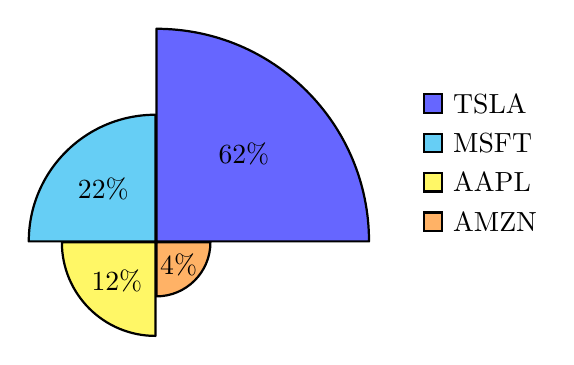
\begin{tikzpicture}[scale=0.9]
    \pie[polar, explode=0.01, text=legend]
    {62/TSLA, 22/MSFT, 12/AAPL, 4/AMZN}
  \end{tikzpicture}
\end{minipage}%
\begin{minipage}{0.6\textwidth}
  \[
  \mathbf{\omega} = \begin{bmatrix} \omega_0 \\ \omega_1 \\ \omega_2 \\ \omega_3 \end{bmatrix} = \begin{bmatrix} 0.62 \\ 0.22 \\ 0.12 \\ 0.04 \end{bmatrix} \rightarrow \begin{bmatrix} 62\% \rightarrow \text{Tesla} \\ 22\% \rightarrow \text{Microsoft} \\ 12\% \rightarrow \text{Apple} \\ 4\% \rightarrow \text{Amazon} \end{bmatrix}
  \]
\end{minipage}
\\~\\

\noindent
Finally given \textit{G} we can calculate the budget allocated for each asset by simply multiplying \textit{G} with $\bm{\omega}$. One can then calculate the numbers of shares they can buy. Since most modern investment platforms allow the users to buy fractional shares, the number of shares is calculated as a simple division of the budget allocated for this specific asset and the asset price.
\[
\text{number of shares} = G \cdot \bm{\omega} \div \text{asset price}
\]

\newpage

\noindent
\textbf{\underline{Definition of risk and return}}
\\~\\
We define the daily return \(dr_i^{(t)}\) and the daily growth factor \(dgf_i^{(t)}\) of an investment in asset \textit{i} at timestamp \textit{t} as:
\begin{align*}
dr_i^{(t)} &= \frac{p_i^{(t)} - p_i^{(t-1)}}{p_i^{(t-1)}} & dgf_i^{(t)} &= dr_i^{(t)} + 1
\end{align*}

\noindent
The cumulative return \(cr_i\) is calculated simply by multiplying all daily growth factors for the whole timeline that consists of \textit{D} days. The annualized return \(r_i\) depends on the number of days \textit{n} in the year the asset was held. For simplicity we assume that we perform long term investments, and therefore set \(n=D\).
\begin{align*}
cr_i &= \prod_{t=1}^{D} dgf_i^{(t)} & r_i &= cr_i^{\frac{D}{n}} - 1
\end{align*}
\noindent
The risk taken by the investor in the portfolio is measured by the volatility \(\sigma= \sqrt{\omega^T \Sigma \omega}\), which is computed from the covariance matrix \textbf{$\Sigma$}. The covariance matrix is a matrix that captures the variance and covariance among multiple variables (here assets). It provides a measure of how changes in one variable might be associated with changes in another. Let's define $\bm{a_i}$ as a vector of daily returns of each asset \textit{i}:
\begin{align*}
\bm{a_i} &= [dr_i^1, dr_i^2, dr_i^3, \dots, dr_i^D] & E[\bm{a_i}] &= \frac{1}{D} \sum_{t=1}^{D} dr_i^t
\end{align*}

\noindent
The variance and covariance of asset \(i\) is defined as:
\begin{align*}
\text{var}(\bm{a_i}) &= \frac{1}{D} \sum_{t=1}^{D} (dr_i^t - E[\bm{a_i}])^2 & \text{cov}(\bm{a_i}, \bm{a_j}) &= \frac{1}{D} \sum_{t=1}^{D} \left( (dr_i^t - E[\bm{a_i}]) \cdot (dr_j^t - E[\bm{a_j}]) \right)
\end{align*}


\[
\bm{\Sigma} = \begin{bmatrix}
\text{var}(\bm{a_0}) & \text{cov}(\bm{a_0}, \bm{a_1}) & \dots & \text{cov}(\bm{a_0}, \bm{a_N}) \\
\text{cov}(\bm{a_1}, \bm{a_0}) & \text{var}(\bm{a_1}) & \dots & \text{cov}(\bm{a_1}, \bm{a_N}) \\
\vdots & \vdots & \ddots & \vdots \\
\text{cov}(\bm{a_N}, \bm{a_0}) & \text{cov}(\bm{a_N}, \bm{a_1}) & \dots & \text{var}(\bm{a_N})
\end{bmatrix}
\]

\begin{figure}[H]
    \centering
    \begin{subfigure}[b]{0.45\textwidth}
        \includegraphics[width=\textwidth]{cov_graph_positive.png}
        \caption{Positive covariance}
        \label{fig:image1}
    \end{subfigure}
    \hfill % ensures both subfigures are aligned to the page edges
    \begin{subfigure}[b]{0.45\textwidth}
        \includegraphics[width=\textwidth]{cov_graph_negative.png}
        \caption{Negative covariance}
        \label{fig:image2}
    \end{subfigure}
    \caption{Description of covariance.}
    \label{fig:group}
\end{figure}

\newpage

\section{QUBO Formulation of the Problem}

\noindent
The optimal portfolio \cite{main_portfolio} is one that maximizes reward and minimizes risk. Each maximization problem can turn into a minimization problem by just flipping the sign. The optimal portfolio therefore minimizes the cost function:

\[ C(\boldsymbol{\omega}) = -\mathbf{r}^T \boldsymbol{\omega} + \frac{\gamma}{2} \boldsymbol{\omega}^T \mathbf{\Sigma} \boldsymbol{\omega} \]

\noindent
In this equation, the vector \(\mathbf{r}\) is the vector of annualized returns and the parameter \(\gamma\) is the so-called risk aversion, which controls the portfolio's penalty for risk. As it is obvious, increasing risk aversion translates to a decreased amount of risk the investor is willing to take. Both the covariance matrix and the vector of returns are precalculated by the collected stock data. In practice, we also want to fix the entire budget being invested to a constant (defined as \( \textit{G} \) previously). This means that the \textbf{omega vector} must be \textbf{normalized}. We can achieve this by adding a penalty constraint to the cost function controlled via a Lagrangian multiplier:

\[
C(\boldsymbol{\omega}) = -\mathbf{r}^T \boldsymbol{\omega} + \frac{\gamma}{2} \boldsymbol{\omega}^T \mathbf{\Sigma} \boldsymbol{\omega} + \rho \left( \sum_{i=0}^{N} \omega_i - 1 \right)^2
\]

\noindent
In real life settings, financial institutions construct a variety of portfolios for different risk profiles. The problem then is to obtain the best possible portfolio, i.e., the one that maximizes returns, for a given value of the risk as measured by the portfolio’s volatility. There are two ways we can achieve this. One is to perform the calculation for different values of the risk aversion \( \frac{\gamma}{2} \) to obtain different values of volatility and then choose the one that suits us. This method is arguably very inefficient. The other way is to force the cost function by introducing another constraint controlled via a Lagrangian Multiplier.

\[
C(\boldsymbol{\omega}) = -\mathbf{r}^T \boldsymbol{\omega} + \rho \left( \sum_{i=0}^{N} \omega_i - 1 \right)^2 + \tau (\boldsymbol{\omega}^T \mathbf{\Sigma} \boldsymbol{\omega} - \sigma_{\text{target}}^2)^2
\]

\noindent
Finally we need to also integrate investment bands into the model. In simple words, this means that there is a minimum and a maximum investment for each asset. The reason we need this is because it enforces diversification in the portfolio, so as to avoid possible corner solutions, like for example portfolios where most of the budget is allocated in only a few assets. These solutions, even if mathematically correct, are not wanted because there are other factors (environmental e.t.c.) that cannot be modeled and may affect the course of a company. Also some companies allow investments only in large bundles, meaning that they set a minimum investment. Mathematically speaking this means that omega is bounded by a minimum and a maximum value.

\[ \omega_i \in [\omega_i^{\text{min}}, \omega_i^{\text{max}}] \subset \mathbb{R} \]

\noindent
We can, however perform a linear transformation so that counting starts from 0 instead of an arbitrary number. This will come handy later as it is much easier to count in binary numbers starting from 0. Note that it is also very easy to retrieve the original $\omega_i$ variables by performing the linear transformation in reverse.

\[
\tilde{\omega}_i = \omega_i - \omega_i^{\text{min}} \implies \tilde{\omega}_i \in [0, \omega_i^{\text{max}} - \omega_i^{\text{min}}]
\]

\newpage
\noindent
\textbf{\underline{Discretizing $\omega_i$}}
\\~\\

\noindent
The variables $\tilde{\omega}_i$ are discretized by using binary variables. This implies that investments come in discrete packets. Also, by using a fixed number of bits for each $\tilde{\omega}_i$ variable, a natural upper cutoff is implemented making the process of counting much easier. The encoding we use for this particular case is:

\[
\tilde{\omega}_i = \frac{1}{K} \left( \sum_{q=0}^{B_i-1} 2^q x_{i,q} + M \cdot x_{i,B_i} \right)
\]

\begin{itemize}
    \item $x_{i, q} \in \{0, 1\}$ is the readout value of the $q^{\text{th}}$ qubit assigned to asset $i$.
    \item $K$ is a constant and represents the resolution of the discretization.
    \item $M = K \cdot (\omega_i^{\text{max}} - \omega_i^{\text{min}}) - (2^{B_i -1} - 1) \geq 0$ is a constant representing overflow offset.
    \item $B_i = 1 + \left\lfloor \log_2 \left(1 + K \cdot (\omega_i^{\text{max}} - \omega_i^{\text{min}}) \right) \right\rfloor$ is the number of bits used per $\omega_i$
\end{itemize}

\noindent
The above expression of \(\tilde{\omega}_i\) can be simplified when \(K\) is one less than a power of 2 (\(K = 2^k - 1\)). The simplified expression is:

\[
\tilde{\omega}_i = \frac{1}{K} \sum_{q=0}^{2^k} 2^q x_{i,q}
\]
\\
\noindent
\textbf{Treating the bitvector as an unsigned integer}, it is now clear how this formulation works. Below is a table that demonstrates counting in discrete steps and shows the resulting $\tilde{\omega}_i$ variable for $K=4$.

\begin{table}[h!]
\centering
\begin{tabular}{|c|c|}
\hline
\textbf{Bitstring} & \boldmath{$\tilde{\omega}_i$} \\
\hline
0000 & 0.00 \\
\hline
0001 & 0.07 \\
\hline
0010 & 0.13 \\
\hline
0011 & 0.20 \\
\hline
0100 & 0.27 \\
\hline
0101 & 0.33 \\
\hline
0110 & 0.40 \\
\hline
0111 & 0.47 \\
\hline
1000 & 0.53 \\
\hline
1001 & 0.60 \\
\hline
1010 & 0.67 \\
\hline
1011 & 0.73 \\
\hline
1100 & 0.80 \\
\hline
1101 & 0.87 \\
\hline
1110 & 0.93 \\
\hline
1111 & 1.00 \\
\hline
\end{tabular}
\end{table}

\noindent
If the resolution \( K \) is not a power of 2, then things get a bit more complicated. This is where the constant \( M \) is used. By replacing the coefficient of the most significant bit with \( M \), the counting process can be manipulated to always reach the desired \( \tilde{\omega}_i^{\text{max}} \) when all bits are 1. Overall, this is a great encoding that uses linear binary terms for each \( \tilde{\omega}_i \) variable. This means that \( \tilde{\omega}_i^2 \) will produce quadratic binary variables, which is on the right path of transforming this problem into QUBO.
\\

\noindent
To finally turn the problem into QUBO, we have to slightly change the cost function. Since it is now clear that the binary representation of the cost function will be a polynomial of the same rank as the initial expression, there is one constraint in the cost function that poses a problem, which is:

\[ \tau (\boldsymbol{\omega}^T \mathbf{\Sigma} \boldsymbol{\omega} - \sigma_{\text{target}}^2)^2 \]

\noindent
Notice how this term contains \(4^{\text{th}}\) order polynomial \(\omega_i^4\) terms. This means that the binary mapped equivalent constraint from the mapping we showed earlier will have \(4^{\text{th}}\) order polynomial binary terms. Problems of this type are referred to as HUBO (Higher order Unconstraint Binary Optimization). Solving such problems is known to be quite complicated since they involve order reduction techniques with a substantial number of overhead bits. In order to avoid this unpleasant and non-optimal situation as well as increasing the number of binary variables and yet be able to impose the constraint, we will linearize the portfolio covariance:

\[ \tau (\boldsymbol{k}^T \mathbf{\Sigma} \boldsymbol{\omega} - \sigma_{\text{target}}^2)^2 \]

\noindent
Here \( k \) is a vector of constants usually referred to as linear weights. This linearization implies that the constraint remains quadratic, but at the price of having to find \( k \) somehow. Different options are possible, like optimizing \( k \) in some tensor network algorithms \cite{Tensor}. Another option is to fine-tune \( k \) starting from a suitable approximation like for example:
\[ k_i = \frac{1}{N} \text{ for each asset } i. \]
Note that, for the purpose of simplicity, the \( k \) vector will remain untouched in the following experiments. The final cost function is:

\[
C(\boldsymbol{\omega}) = -\mathbf{r}^T \boldsymbol{\omega} + \rho \left( \sum_{i=0}^{N} \omega_i - 1 \right)^2 + \tau (\boldsymbol{k}^T \mathbf{\Sigma} \boldsymbol{\omega} - \sigma_{\text{target}}^2)^2
\]

\[ \omega_i = \tilde{\omega}_i + \omega_i^{\text{min}} \]

\[
\tilde{\omega}_i = \frac{1}{K} \left( \sum_{q=0}^{B_i-1} 2^q x_{i,q} + M \cdot x_{i,B_i} \right)
\]
\\
\noindent
Since the problem is now correctly formulated as a QUBO, we can go ahead and implement it on a quantum computer. However, the number of binary variables is \(O(N \log K)\). With \(K=100\) i.e. \(0.01\) resolution, which is a reasonable number, the number of binary variables and, as a result, the number of qubits increases as \(\approx 7 \times N\). Even a toy problem where \(N=4\) would require approximately 28 qubits. For this reason, this problem will be executed only on D-wave annealers which can handle up to 5000 qubits, since using QAOA or hardware-efficient VQA is futile.


\newpage

\section{Implementing on D-Wave Quantum Annealer}
Each part of the model will be tested separately to make sure the behavior of the quantum computer is as expected and possibly figure out any limitations. At the end, the entire model will be executed using the Hybrid Binary Unconstrained Solver provided also by D-Wave that can handle a lot more variables. The cost function is separated into 3 parts:

\[ C_1(\omega) = -r^T \cdot \omega \]

\[ C_2(\omega) = \rho \cdot \left( \sum_{i=0}^{N} \omega_i - 1 \right)^2 \]

\[ C_3(\omega) = \tau \cdot \left( k^T \Sigma \omega - \sigma_{\text{target}}^2 \right)^2 \]

\noindent
\textbf{\underline{Testing term $1$}}
\\~\\

\noindent
For this experiment we consider the average return of \textbf{AAPL}, \textbf{MSFT}, \textbf{NVDA}, and \textbf{TSLA} from 01-01-2020 to 01-01-2023. The symbols highlited in bold are called tickers and correspond to Apple, Microsoft, Nvidia and Tesla accordingly. The vector of average annualized return is:

\[ \mathbf{r} = 
\begin{bmatrix}
r_{\text{AAPL}} \\
r_{\text{MSFT}} \\
r_{\text{NVDA}} \\
r_{\text{TSLA}}
\end{bmatrix}
=
\begin{bmatrix}
0.102 \\
0.081 \\
0.180 \\
0.296
\end{bmatrix} \]

\noindent
The goal is to minimize the cost function \( C_1(\omega) = -\mathbf{r}^T \omega \). There are \( N = 4 \) assets (those described above) and we set \( \omega^{\text{max}} = 1 \) and \( \omega^{\text{min}} = 0 \). The resolution is set to \( K = 10^5 \). This means that we have 15 qubits per asset, totalling 60. Note that this is a trivial problem, since the cost function is linear and the minimum is very easy to compute. The values that minimize \( C_1(\omega) \) are \( \omega = [1, 1, 1, 1] \) and that is true because \(r>0\) for every \(i\). This means that the binary variables should all be 1, because of the expression:

\[
\tilde{\omega}_i = \frac{1}{K} \left( \sum_{q=0}^{B_i-1} 2^q x_{i,q} + M \cdot x_{i,B_i} \right)
\]

\noindent
The cost function is minimized in a quantum annealer. Since there are no quadratic terms here, the qubits do not interact with each other and they are only subject to their bias. We perform the minimization a total of \(100\) times. Each experiment performs \(100\) runs and the total annealing time per run is \(20 \mu s\). We count the number of times each variable was measured to be \(1\) and then we average out by all the number of measurements. Finally, each qubit's probability is plotted in a diagram. If the result is \(0.8\) for a qubit, for example, this means that in all experiments and all measurements this particular qubit was '1' \(80\%\) of the time.




\begin{figure}[!h]
    \centering
    \includegraphics[width=0.55\textwidth]{term_1_experiment_cmap.png} 
    \caption{Average probabilities of qubits among 100 experiments with 100 measurements per experiment with 20 us annealing time (\(K=10^5\)). The expected readout result of binary variables should be all '1'.}
    \label{fig:cmap_term_1}
\end{figure}

\newpage

\noindent
Notice how most significant bits (right) have a higher tendency of being one than least significant bits (left). In fact, measurement results from bits \(0\) to \(6\) are considered pure noise since their average tendency is close to \(0.5\). The reason for this is that the bias decreases exponentially when moving from most significant to least significant bits. Interestingly enough, we can predict the sequence of the biases from smallest to largest, just by watching how fast the tendency decays. However, the deviation from the expected correct result is very small, even though most readout results in the least significant bits are noisy. This is because the least significant bits do not affect the result of the \(\omega\) variables that much. This should provide insight into why we should not increase \(K\) too much. A more modest value, like \(K=100\), should work just as well.

\begin{figure}[h]
    \centering
    \includegraphics[width=0.9\textwidth]{term_1_performance.png} 
    \caption{The sum of all \(\omega\) variables, \(\sum_{i=0}^{3} \omega_i\), is used as a measure of the quality of the solution. We are expecting all \(\omega_i\) variables to be equal to one, and therefore the total sum should be 4. We can see that despite the random behavior of the least significant bits, the quality of the solution is still good.}
    \label{fig:per_term_1}
\end{figure}

\newpage
\noindent
\textbf{\underline{Testing term $2$}}
\\~\\

\noindent
The goal of this test is to check whether or not the constraint \(C_2(\omega)\) is implemented correctly. Note that 
\[ C_2(\omega) = \rho \left( \sum_{i=0}^{N} \omega_i - 1 \right)^2 \]
\noindent
It is very easy to see that this function is minimized when the sum of \(\omega_i\) variables is equal to \(1\). We can therefore use this as a measure of the accuracy. In this benchmark we consider \(N=6\). Although it doesn't matter, we chose `TSLA', `AMZN', `AAPL', `MSFT', `GOOGL', and `NVDA'. The \(\omega^{\text{max}}\) is set to \(1\) and the \(\omega^{\text{min}}\) is set to \(0\). The resolution is set to \(K=100\), meaning that there are \(7\) binary variables per asset, totalling \(42\) binary variables. We perform a total of \(20\) experiments with \(100\) measurements per experiment. From those measurements, we select the one with the "minimum energy" which is returned by the annealer. We plot the cumulative sum of the \(\omega_i\) variables of the best answer per \(100\) measurements (top \(1\%\)) in each experiment, as well as the ideal result. Finally, we do this for \(20 \mu s\) and \(2 \text{ms}\) annealing time to see if there is any difference between them.


\begin{figure}[!h]
    \centering
    \includegraphics[width=0.7\textwidth]{constraint_2.png} 
    \caption{Performance tracking of constraint 2. This experiment tracks the result \(\sum_{i=0}^{5} \omega_i\), which must be as close to 1 as possible. Performed a total of 20 experiments with 20 us and 2 ms annealing time.}
    \label{fig:constr_2}
\end{figure}

\noindent
We observe from the results depicted above that the model behaves as expected and the total cumulative sum is really close to \(1\). The annealing time does not seem to have a huge impact on the results, but this may be because the total number of experiments is not enough to make objective conclusions. However, \(2 \text{ms}\) seems to be better, since it's peak deviation is smaller than \(20 \mu s\).
\newpage

\noindent
\textbf{\underline{Testing term $3$}}
\\~\\

\noindent
The goal of this third and final test is to check whether or not the target volatility constraint is implemented correctly:
\[ C_3(\omega) = \tau \left( \mathbf{k}^T \Sigma \omega - \sigma_{\text{target}}^2 \right)^2 \]
We start by setting \(N=6\) (the same assets as the previous experiment) and \(K=100\). Next, we minimize \(C_3(\omega)\) given several different values of \(\sigma_{\text{target}}^2\): [0, 0.15, 0.20, 0.25, 0.30, 0.40, 0.50, 0.70]. For each of these values, we perform 10 experiments with 400 measurements per experiment with an annealing time of \(200 \mu s\). We once again select the answer with the minimum energy which represents the top \(0.25\%\) of the answers. Finally, after the annealing process, we compute, given the best result, the return and volatility, and we plot them in figure \ref{fig:tgt_volatility}.

\begin{figure}[!h]
    \centering
    \includegraphics[width=1\textwidth]{tgt_volatility_experiments.png} 
    \caption{Benchmark of the accuracy of finding the target volatility \(N=6\) and \(K=100\).}
    \label{fig:tgt_volatility}
\end{figure}

\noindent
The \(x\)-axis of the left graph is the linearized volatility, which corresponds to the actual value that was targeted. We observe that most measurements are really accurate with the exception of target volatilities greater than \(60\) or smaller than \(20\). This is probably due to the fact that this specific portfolio simply cannot produce such volatilities. 
\\

\noindent
The \(x\)-axis of the right graph shows the actual volatility. Notice how results are skewed from the initial target. This is due to the linearization of the volatility that we performed earlier to transform the problem into QUBO. The shift, however, seems to be linear and does not distort the target volatility that much, meaning that we might be able to purposely change \(\sigma_{\text{target}}^2\) to accommodate for this error.

\newpage
\noindent
\textbf{\underline{Scalability}}
\\~\\
Scalability is very important factor that determines any limits in the number of variables we can run on the annealer. It seems like \(140\) variables is the limit, where no accurate solutions can be extracted for constraints \(C_2(\omega)\) and \(C_3(\omega)\). The reason for this is that the \(J\) matrix of the Ising Hamiltonian of these constraints is fully connected. This poses a serious challenge, as shown by the following image, that we are limited by either \(K=10^5\) and \(N=10\) or \(K=100\) and \(N=20\). These values are toy models and not real-world scenarios. For this reason, we need to deviate from pure quantum annealing and use D-wave's Hybrid Quantum Solver which utilizes heuristic methods in combination with the annealer.

\begin{figure}[!h]
    \centering
    \includegraphics[width=0.95\textwidth]{qpu_zommed.png} 
    \caption{Quantum Processing Unit (QPU - Advantage) usage for \(K=10^5\) and \(N=10\). The total number of binary variables is 140, but the total number of qubits used is 2833 out of 5760, which translates to 49.18\%. The topology of the processor (each qubit connected with 16 others) limits the scalability of the initial problem (which is fully connected). To resolve this, chains of maximally coupled qubits are created which represent only one binary variable (marked with blue).}
    \label{fig:qpu}
\end{figure}



\newpage

\section{Quantum Amplitude Encoding for VQA}

This is a new method for this specific problem we developed in the context of this thesis, that aims to fix some major issues. The main motivation is that the initial problem is not binary. Converting it to QUBO we deal with a lot of issues like having a lot of binary variables and potentially not getting valid results when \(N\) is really high. Also violating constraint \(C_2\) gives us wrong answers. Notice how we can encode the \(\omega_i\) variables directly into the statevector. This method is called \textbf{amplitude encoding} and although it already exists this new method has a slight variation that is adapted for this specific problem. Mathematically we can express the statevector as:

\[
\ket{\psi} = \sum_{i=0}^{N} \sqrt{\omega_i} \ket{i}
\]
\\
\noindent
Notice that the statevector must be normalized. This is a fundamental property of a quantum system. The probability of measuring a state \(\ket{i}\) gives us the \(\omega_i\) variable:

\[
Pr(\ket{i}) = \omega_i
\]
\\
\noindent
We are guaranteed that \(\sum_{i=0}^{N} \omega_i = 1\), meaning that we can completely remove constraint \(C_2(\omega)\) from the cost function. The new cost function is:

\[
C(\omega) = -r^T \cdot \omega + \tau \left( \omega^T \Sigma \omega - \sigma_{\text{target}}^2 \right)^2
\]
\\
\noindent
Notice how since the statevector doubles in size each time we add a qubit, the number of qubits grows logarithmically with the input number of assets \(N\).

\[
n_{\text{qubits}} = O(\log_2(N))
\]
\\
\noindent
Although this may seem good at first, it is highly unlikely that we will be able to reach all states. We cannot use QAOA or annealing here, since the problem has not been converted into energy minimization. The only viable algorithm we can use is the hardware efficient VQA. We already talked about barren plateaus in this algorithm. The combination of this with the fact that we only have a logarithmic number of optimization variables (\(L\) for each qubit), where \(L\) is the number of layers, makes it very unlikely to find good solutions among the possible statevectors. Another major problem is that we cannot force diversification.
\\
\\
\noindent
Luckily we can solve both problems by splitting the initial circuit into 2 circuits with combined statevector size equal to the number of assets \(N\). This means that by using, let's say, \(n\) qubits initially to encode all the \(\omega\) variables into a single statevector, we can now encode \(N/2\) \(\omega\) variables into 2 statevectors. The number of qubits this way increases from \(n\) to \(2n-2\) (see Figures \ref{fig:amp_enc_split_0} \ref{fig:amp_enc_split_1}). For example, if we want to find the optimal portfolio among \(N=128\) assets initially we would have:

\[
\ket{\psi} = \sum_{i=0}^{127} \sqrt{\omega_i} \ket{i}
\]

\noindent
By splitting the statevector into 2 different statevectors we would have:

\[
\ket{\psi} = \ket{\psi_1} \otimes \ket{\psi_2} = \sum_{i=0}^{63} \sqrt{\omega_i} \ket{i} \otimes \sum_{j=64}^{127} \sqrt{\omega_j} \ket{j-64}
\]
\\
\noindent
Upon measurement of the system, we essentially obtain 2 \(\omega_i\) variables. This implies that the accuracy of the final measurement increases exponentially, which is also very good. Other than that each individual circuit has its own normalized statevector. This means that:

\[
\sum_{i=0}^{63} \omega_i = \sum_{j=64}^{127} \omega_j = 1
\]
\\
\noindent
We can further normalize the combined \(\omega\) result by dividing by 2. Notice that we created a natural barrier of \(\omega_i^{\text{max}} = 0.5\) and we don't need to encode any extra penalty constraints.
\\
\\
\noindent
We can further generalize this to any arbitrary number of splits \(S\) and examine the behavior of \(\omega^{\text{max}}\) and the total number of qubits used. Since in each split the number of qubits used per individual circuit decreases by 1 and the total number of individual circuits doubles, the total number of qubits used is:

\[
n_{\text{qubits}} = (\log_2N - S) \cdot 2^S
\]
\\
\noindent
The \(\omega^{\text{max}}\) exponentially decreases with each splitting of the statevector, meaning that:

\[
\omega^{\text{max}} = \frac{1}{2^S}
\]
\\
\noindent
This implies that with 3 splittings for example and \(N=128\) assets we would have 32 total qubits and the upper bound for an \(\omega\) variable would be \(\frac{1}{8} = 0.125\) which is a pretty good diversification barrier.
\\

\noindent
Although both initial problems were solved, notice that we still cannot force a lower barrier \(\omega^{\text{min}}\). This is not a huge issue though, since most well-known companies in well-known markets like the US market do not require a minimum investment to sell their stocks. Finally, notice that the correlation of the \(\omega_i\) variables decreases exponentially, since fewer qubits can be entangled, and therefore fewer entangled states can be generated. This is fine though (as demonstrated by the experiments that follow) as keeping \(S\) low will ensure a balance between the number of entangled states and diversification.

\newpage

\begin{figure}[!h]
    \centering
    \includegraphics[width=0.6\textwidth]{amp_split_0.png}
    \caption{Amplitude encoding for \(N=128\) and \(S = 0\). In this scenario, the number of qubits is 7.}
    \label{fig:amp_enc_split_0}
\end{figure}

\begin{figure}[!h]
    \centering
    \includegraphics[width=0.6\textwidth]{amp_split_1.png}
    \caption{Amplitude encoding for \(N=128\) and \(S=1\). In this scenario, the number of qubits used is 12. Notice how the circuit can be split into 2 smaller circuits, since there is no entangling gate between qubit \(q_5\) and qubit \(q_6\).}
    \label{fig:amp_enc_split_1}
\end{figure}

\newpage

\section{Results}

\noindent
\textbf{\underline{Amplitude Encoding VQA}}
\\

\noindent
The next experiments were executed using the hardware efficient VQA on a quantum simulator. The hyperparameter \(\tau=10^3\) and the number of assets is \(N=128\) with \(\omega^{\text{max}}=0.125\), \(\omega^{\text{min}}=0\) and \(S=3\). The total number of qubits used is 32 and the number of layers is \(L=2\). There are 10000 shots per circuit execution. The optimization is performed for target volatilities \(10\%\), \(16\%\), and \(20\%\), with 20 experiments per \(\sigma_{\text{target}}^2\). In Figure \ref{fig:meas_results}, we see on the right column the optimized portfolios and on the left column we see the average cost evolution.


\begin{figure}[!h]
    \centering
    \includegraphics[width=1\textwidth]{experimental_results_amp_encoding.png}
    \caption{Portfolio optimization for target volatility $10\%$, $16\%$, and $20\%$ in the first, second, and third row accordingly.}
    \label{fig:meas_results}
\end{figure}

\newpage

\begin{figure}[!h]
    \centering
    \includegraphics[width=0.8\textwidth]{final_result_sandp128.png}
    \caption{Comparison between average optimized portfolios for $N=128$ stocks selected from S\&P500 companies and $\omega^{\text{max}} = 0.125$ for each stock. We see that the optimized results tend to create a line of ``Optimal Portfolios'' as described earlier (see Figure \ref{fig:portfolio}). We also observe that target volatility $10\%$ is skewed a lot. That makes sense, since the dataset is from 01-01-2020 to 01-01-2023 and during the pandemic there was a lot of variance in the stock market.}
    \label{fig:concl_results}
\end{figure}

\begin{figure}[!h]
    \centering
    \includegraphics[width=0.8\textwidth]{sectors_20.png}
    \caption{Sector Distribution of the average optimized portfolio for $20\%$ target volatility. We can see that with $3$ splits and $\omega^{\text{max}} = 0.125$ the optimized portfolio is diversified.}
    \label{fig:sec_20}
\end{figure}

\newpage

\noindent
\textbf{\underline{Hybrid Quantum Annealer}}
\\

\noindent
The next experiments were executed on D-Wave - Hybrid Solver. The hyperparameter values are $\rho=1$, $\tau=10^3$. The number of assets is $N=128$ with $\omega^{\text{max}}=0.125$ and $\omega^{\text{min}}=0$. The total execution time was 15 seconds (hybrid time: classical and quantum).


\begin{table}[h]
    \renewcommand{\arraystretch}{1.5} % Adjusts the row height
    \centering
    \begin{tabular}{|c@{\hspace{1cm}}|c@{\hspace{1cm}}|c@{\hspace{1cm}}|c@{\hspace{1cm}}|c|}
        \hline
        \textbf{$\sigma_{\text{target}}$ (\%)} & \textbf{$\sum_{i=0}^{N} \omega_i$} & \textbf{$\sqrt{k^T \Sigma \omega}$} & \textbf{$\sqrt{\omega^T \Sigma \omega}$} & \textbf{$r^T\omega$} \\
        \hline
        10 & 0.974 & 0.134 & 0.138 & 0.124 \\
        \hline
        16 & 1.007 & 0.166 & 0.192 & 0.175 \\
        \hline
        20 & 1.085 & 0.197 & 0.271 & 0.197 \\
        \hline
    \end{tabular}
    \caption{Results of constraints for different risk profiles.}
    \label{tab:Dwave-results}
\end{table}

\begin{figure}[h]
    \centering
    \includegraphics[width=1\linewidth]{dwave-results.png}
    \caption{Comparison between linearized and actual annual volatility results after optimization}
    \label{fig:dwave-plots}
\end{figure}

\newpage

\chapter{Conclusion and Future Work}

\noindent
Our results demonstrate that quantum computers could be effectively utilized for solving real-world applications, particularly in finance. We tried different implementations of quantum approches, including quantum annealing and variational algorithms,  and the results where consistent with our predictions, indicating good performance of a range of parameters. However, it is crucial to highlight that we did not compare our outcomes with existing classical methods for addressing such challenges due the early stages of available clould quantum hardware at the moment. Although classical optimization techniques might at the moment still surpass our results, it’s encouraging to observe that quantum computers can in principle tackle such problems, with the potential to surpass classical machines in the not so distant future (tens of thousands of qubits compared to the few hundred available now). The fundamental different way of processing information at the quantum level, the potential for major speed ups in certain applications, make working in this field an exciting endeavour.
\\

\noindent
After we introduced the basic tools of quantum quantum computing and quantum optimization in chapters 1 and 2, in chapter 3, we addressed two separate mathematical problems, the Subset Sum and the Travelling Salesman Problem and carried out tests to contrast the different quantum optimization methods. Even though QAOA is asymptotically superior to VQA, contemporary use cases seem to derive greater benefits from the hardware-efficient VQA since it is more robust and less susceptible to noise. We observed that D-Wave’s quantum annealers, along with their hybrid solvers, currently stand out as the most effective methods for optimization challenges. In collaboration with Prof. Angelakis and industry partners, I am currently exploring various R \& D projects in this direction in the field of quantum optimization, which will be an exciting follow up to this work.
\\

\noindent
As we delve deeper into the intricacies of quantum computing, there's a promising avenue to further explore the formulation of optimization problems using QUBO and their execution on quantum platforms. One notable area of interest is route optimization, which holds immense significance in global commerce. By optimizing routes, industries stand to reap substantial time and cost savings, especially in the domains of transportation and logistics. Another crucial aspect is scheduling, a facet integral to a vast range of sectors from manufacturing plants to service industries. Efficient scheduling can be a game-changer in enhancing productivity and optimal resource allocation. Additionally, the realm of resource management optimization presents itself as a potential goldmine of research opportunities. Whether it's human resources, material assets, or financial allocations, effective resource management can drastically influence an organization's profitability and operational efficiency.
\\

\noindent
Interestingly, the global corporate landscape is buzzing with curiosity about quantum computing. Numerous enterprises are keen to assess the capabilities of quantum computers in possibly providing faster solutions or even superior alternatives to their existing problem-solving methodologies. Collaborating with such businesses in our subsequent research endeavors could not only present us with tangible real-world challenges but also enable a practical evaluation.
\\

\noindent
It’s safe to say that we’ve entered the quantum era. Quantum computers have become increasingly accessible through cloud services, and their popularity continues to grow with rising investments. Leading commercial producers, primarily IONQ and D-Wave, are making promising strides in fault-tolerant hardware and optimization-centric hardware respectively. Nonetheless, algorithms with established enhancements, such as Shor’s or Grover’s, might remain elusive for some years to come

\appendix

\chapter{Mathematical Proofs}
\newtheorem{proof}{Proof}
\begin{proof}
\textbf{Subset sum cost function to Ising Hamiltonian.}
\[C(x) = \left(\sum_{i=0}^{N} a_i \cdot x_i - S\right)^2 = \left(\sum_{i=0}^{N} a_i \cdot x_i\right)^2 - 2S \left(\sum_{i=0}^{N} a_i \cdot x_i\right) + S^2\]

\[C(x) = \sum_{i=0}^{N} \sum_{j=0}^{N} a_i \cdot a_j \cdot x_i \cdot x_j - \sum_{i=0}^{N} \left(2S \cdot a_i \cdot x_i\right) + S^2\]

    \begin{center}
    Next we substitute \(x_i = \frac{s_i + 1}{2}\) in the equation.
    \end{center}

\[C(s) = \sum_{i=0}^{N} \sum_{j=0}^{N} a_i \cdot a_j \cdot \frac{{s_i + 1}}{2} \cdot \frac{{s_j + 1}}{2} - \sum_{i=0}^{N} \left(2S \cdot a_i \cdot \frac{{s_i + 1}}{2}\right) + S^2\]

\[C(s) = \frac{1}{4} \sum_{i=0}^{N} \sum_{j=0}^{N} a_i \cdot a_j \cdot (s_i + 1) \cdot (s_j + 1) - S \sum_{i=0}^{N} a_i \cdot (s_i + 1) + S^2 \]

\[C(s) = \frac{1}{4} \sum_{i=0}^{N} \sum_{j=0}^{N} a_i \cdot a_j \cdot (s_i \cdot s_j + s_i + s_j + 1) - S \sum_{i=0}^{N} (a_i \cdot s_i + a_i) + S^2 \]

\[C(s) = \frac{1}{4} \sum_{i=0}^{N} \sum_{j=0}^{N} (a_i \cdot a_j \cdot s_i \cdot s_j + a_i \cdot a_j \cdot s_i + a_i \cdot a_j \cdot s_j + a_i \cdot a_j) - S \sum_{i=0}^{N} a_i \cdot s_i - S \sum_{i=0}^{N} a_i + S^2 \]

\begin{center}
Next we ignore the constant term:
\end{center}

\[ \frac{1}{4} \sum_{i=0}^{N} \sum_{j=0}^{N} a_i a_j - S \sum_{i=0}^{N} a_i + S^2 \]

\begin{center}
After this, the cost function becomes:
\end{center}

\[ C(s) = \frac{1}{4} \sum_{i=0}^{N} \sum_{j=0}^{N} (a_i a_j s_i s_j + a_i a_j s_i + a_i a_j s_j) - S \sum_{i=0}^{N} a_i s_i \]

\begin{center}
Notice the following relations:
\end{center}

\[ \sum_{i=0}^{N} \sum_{j=0}^{N} a_i a_j s_i = \sum_{i=0}^{N} \sum_{j=0}^{N} a_i a_j s_j = K \sum_{i=0}^{N} a_i s_i \]

\begin{center}
where \( K \) is the sum of all numbers:
\end{center}

\[ K = \sum_{i=0}^{N} a_i \]

\begin{center}
Therefore, the equation simplifies to:
\end{center}

\[ C(s) = \frac{1}{4} \sum_{i=0}^{N} \sum_{j=0}^{N} a_i a_j s_i s_j - (S - \frac{K}{2}) \sum_{i=0}^{N} a_i s_i \]

\begin{center}
Finally, we can further simplify this equation because \( J_{ij} \) and \( J_{ji} \) are equal, and therefore we can add them together:
\end{center}

\[ C(s) = \frac{1}{2} \sum_{i=0}^{N} \sum_{j=i+1}^{N} a_i a_j s_i s_j - (S - \frac{K}{2}) \sum_{i=0}^{N} a_i s_i \]

\begin{center}
The \( J \) matrix and \( h \) vector obtained by this equation are:
\end{center}

\begin{center}
\fbox{
\begin{minipage}{0.7\textwidth}
\[ J_{ij} = \frac{1}{2} a_i a_j, \text{ with } N > i > j \geq 0 \]
\[ h_i = -a_i (S - \frac{K}{2}), \text{ with } N > i \geq 0 \]
\end{minipage}
}
\end{center}

\end{proof}

\newpage


\begin{proof}
\textbf{Linear return term to Ising Hamiltonian.}

\noindent\begin{minipage}{.45\textwidth}
\[ C_1(\omega) = -r^T \omega = - \sum_{i=0}^{N} r_i \omega_i \]
\end{minipage}%
\begin{minipage}{.55\textwidth}
\[ \omega_i = \frac{1}{K} \left( \sum_{q=0}^{B_i - 1} 2^q x_{i, q} + M_i x_{i, B_i} \right) \]
\end{minipage}

\begin{center}
Next we substitute \(\omega_i\) in the initial cost function \(C_1(\omega)\) to get:
\end{center}

\[ C_1(x) = - \sum_{i=0}^{N} r_i \cdot \frac{1}{K} \left( \sum_{q=0}^{B_i-1} 2^q x_{i, q} + M_i x_{i, B_i} \right) = - \sum_{i=0}^{N} \sum_{q=0}^{B_i - 1} \frac{r_i}{K} \cdot 2^q x_{i, q} - \sum_{i=0}^{N} \frac{r_i}{K} \cdot M_i x_{i, B_i}\]

\begin{center}
Next we change into spin basis by substituting \(x = \frac{1 + s}{2}\):
\end{center}

\[ C_1(s) = - \sum_{i=0}^{N} \sum_{q=0}^{B_i - 1} \frac{r_i}{K} \cdot 2^q \cdot \frac{1+s_{i, q}}{2} - \sum_{i=0}^{N} \frac{r_i}{K} \cdot M_i \cdot \frac{1+s_{i, B_i}}{2} \]

\begin{center}
Next, we ignore the constant terms to get:
\end{center}

\[ C_1(s) = - \sum_{i=0}^{N} \sum_{q=0}^{B_i - 1} \frac{r_i}{2K} \cdot 2^q \cdot s_{i, q} - \sum_{i=0}^{N} \frac{r_i}{2K} \cdot M_i \cdot s_{i, B_i} \]

\begin{center}
Finally, we can obtain the coefficients \( h_{i, q} \) of the Ising model:
\end{center}

\begin{center}
\fbox{
\begin{minipage}{0.6\textwidth}
\[ 
h_{i, q} = 
\begin{cases} 
-r_i \cdot \frac{1}{2K} \cdot 2^q & \text{if } q \neq B_i \\
-r_i \cdot \frac{1}{2K} \cdot M_i & \text{if } q = B_i 
\end{cases}
\]
\end{minipage}
}
\end{center}
\end{proof}

\begin{proof}
\textbf{Normalization constraint term to Ising Hamiltonian.}

\noindent\begin{minipage}{.45\textwidth}
\[ C_2(\omega) = \rho \left( \sum_{i=0}^{N} \omega_i - 1 \right)^2 \]
\end{minipage}%
\begin{minipage}{.55\textwidth}
\[ \omega_i = \frac{1}{K} \left( \sum_{q=0}^{B_i - 1} 2^q x_{i, q} + M_i x_{i, B_i} \right) \]
\end{minipage}

\begin{center}
First, we break down the square and ignore the constants to get:
\end{center}

\[ C_2(\omega) = \left( \rho \sum_{i=0}^{N} \omega_i \right)^2 - 2 \rho \sum_{i=0}^{N} \omega_i = \rho \sum_{i=0}^{N} \sum_{j=0}^{N} \omega_i \omega_j - 2 \rho \sum_{i=0}^{N} \omega_i \]

\begin{center}
Substituting the expression for \( \omega_i \) and \( \omega_j \) into the equation, we get:
\end{center}

\begin{align*}
C_2(x) = & \rho \sum_{i=1}^{N} \sum_{j=1}^{N} \left[ \frac{1}{K} \left( \sum_{q=1}^{B_i-1} 2^{q-1} x_{i,q} + M_i x_{i,B_i} \right) \cdot \frac{1}{K} \left( \sum_{r=1}^{B_j-1} 2^{r-1} x_{j,r} + M_j x_{j,B_j} \right) \right] \\
& - 2 \rho \sum_{i=1}^{N} \frac{1}{K} \left( \sum_{q=1}^{B_i-1} 2^{q-1} x_{i,q} + M_i x_{i,B_i} \right)
\end{align*}

\begin{align*}
& C_2(x) = \frac{\rho}{K^2} \sum_{i=1}^{N} \sum_{j=1}^{N} \left[ \sum_{q=1}^{B_i-1} \sum_{r=1}^{B_j-1} 2^{q-1} x_{i,q} 2^{r-1} x_{j,r} \right] + \frac{\rho}{K^2} \sum_{i=1}^{N} \sum_{j=1}^{N} \left[ \sum_{q=1}^{B_i-1} M_j x_{j,B_j} 2^{q-1} x_{i,q} \right] \\
& \quad + \frac{\rho}{K^2} \sum_{i=1}^{N} \sum_{j=1}^{N} \left[ \sum_{r=1}^{B_j-1} M_i x_{i,B_i} 2^{r-1} x_{j,r} \right] + \frac{\rho}{K^2} \sum_{i=1}^{N} \sum_{j=1}^{N} M_i x_{i,B_i} M_j x_{j,B_j} \\
& \quad - 2\frac{\rho}{K} \sum_{i=1}^{N} \left[ \sum_{q=1}^{B_i-1} 2^{q-1} x_{i,q} \right] - 2\frac{\rho}{K} \sum_{i=1}^{N} M_i x_{i,B_i}
\end{align*}


\begin{align*}
& C_2(s) = \frac{\rho}{K^2} \sum_{i=1}^{N} \sum_{j=1}^{N} \left[ \sum_{q=1}^{B_i-1} \sum_{r=1}^{B_j-1} 2^{q-1} \frac{s_{i,q}+1}{2} 2^{r-1} \frac{s_{j,r}+1}{2} \right] + \frac{\rho}{K^2} \sum_{i=1}^{N} \sum_{j=1}^{N} \left[ \sum_{q=1}^{B_i-1} M_j \frac{s_{j,B_j}+1}{2} 2^{q-1} \frac{s_{i,q}+1}{2} \right] \\
& \quad + \frac{\rho}{K^2} \sum_{i=1}^{N} \sum_{j=1}^{N} \left[ \sum_{r=1}^{B_j-1} M_i \frac{s_{i,B_i}+1}{2} 2^{r-1} \frac{s_{j,r}+1}{2} \right] + \frac{\rho}{K^2} \sum_{i=1}^{N} \sum_{j=1}^{N} M_i \frac{s_{i,B_i}+1}{2} M_j \frac{s_{j,B_j}+1}{2} \\
& \quad - 2\frac{\rho}{K} \sum_{i=1}^{N} \left[ \sum_{q=1}^{B_i-1} 2^{q-1} \frac{s_{i,q}+1}{2} \right] - 2\frac{\rho}{K} \sum_{i=1}^{N} M_i \frac{s_{i,B_i}+1}{2}
\end{align*}

\begin{align*}
& C(s)=\frac{\rho}{4K^2} \sum_{i=1}^{N} \sum_{j=1}^{N} \left[ \sum_{q=1}^{B_i-1} \sum_{r=1}^{B_j-1} 2^{q-1} \cdot 2^{r-1} \cdot s_{i,q} \cdot s_{j,r} \right] + \frac{\rho}{4K^2} \sum_{i=1}^{N} \sum_{j=1}^{N} \left[ \sum_{q=1}^{B_i-1} \sum_{r=1}^{B_j-1} 2^{q-1} \cdot 2^{r-1} \cdot s_{j,r} \right] \\
& + \frac{\rho}{4K^2} \sum_{i=1}^{N} \sum_{j=1}^{N} \left[ \sum_{q=1}^{B_i-1} \sum_{r=1}^{B_j-1} 2^{q-1} \cdot 2^{r-1} \cdot s_{i,q} \right] + \frac{\rho}{4K^2} \sum_{i=1}^{N} \sum_{j=1}^{N} \left[ \sum_{q=1}^{B_i-1} M_j \cdot 2^{q-1} \cdot s_{j,B_j} \cdot s_{i,q} \right] \\
& + \frac{\rho}{4K^2} \sum_{i=1}^{N} \sum_{j=1}^{N} \left[ \sum_{q=1}^{B_i-1} M_j \cdot 2^{q-1} \cdot s_{i,q} \right] + \frac{\rho}{4K^2} \sum_{i=1}^{N} \sum_{j=1}^{N} \left[ \sum_{q=1}^{B_i-1} M_j \cdot 2^{q-1} \cdot s_{j,B_j} \right] \\
& + \frac{\rho}{4K^2} \sum_{i=1}^{N} \sum_{j=1}^{N} \left[ \sum_{r=1}^{B_j-1} M_i \cdot 2^{r-1} \cdot s_{i,B_i} \cdot s_{j,r} \right] + \frac{\rho}{4K^2} \sum_{i=1}^{N} \sum_{j=1}^{N} \left[ \sum_{r=1}^{B_j-1} M_i \cdot 2^{r-1} \cdot s_{j,r} \right] \\
& + \frac{\rho}{4K^2} \sum_{i=1}^{N} \sum_{j=1}^{N} \left[ \sum_{r=1}^{B_j-1} M_i \cdot 2^{r-1} \cdot s_{i,B_i} \right] + \frac{\rho}{4K^2} \sum_{i=1}^{N} \sum_{j=1}^{N} M_i \cdot M_j \cdot s_{i,B_i} \cdot s_{j,B_j} \\
& + \frac{\rho}{4K^2} \sum_{i=1}^{N} \sum_{j=1}^{N} M_i \cdot M_j \cdot s_{j,B_j} + \frac{\rho}{4K^2} \sum_{i=1}^{N} \sum_{j=1}^{N} M_i \cdot M_j \cdot s_{i,B_i} - \frac{\rho}{K} \sum_{i=1}^{N} \left[ \sum_{q=1}^{B_i-1} 2^{q-1} \cdot s_{i,q} \right] \\
& - \frac{\rho}{K} \sum_{i=1}^{N} M_i \cdot s_{i,B_i}
\end{align*}


\end{proof}

\bibliographystyle{unsrtnat}
\bibliography{references} % This assumes you named your .bib file "references.bib"


\end{document}
